% The TOPtesi class loads the following packets,
% that's why they are commented below with a single %:
% - graphicx
% - babel
% Other packages are explicitly forbidden by TOPtesi manual,
% that's why they are commented below with a double %
\documentclass[
	%cucitura,				% To decomment when the printable version is needed
	%draft,					% Comment after final revision, also hides images
	twoside]				% Print on both side of the page
	{toptesi}				% We'll be using the toptesi class

%%% PACKAGES USAGE

\usepackage[a-1b]{pdfx}		% Pdf format: PDF/A, mandatory for Polito thesis storage
\usepackage[T1]{fontenc}	% Manages accented chars in output
\usepackage[utf8]{inputenc}	% Input encoding, accept accented chars from keyboard
\usepackage{amsmath,amssymb}% Math chars
% \usepackage{graphicx}		% To include external images, loaded by toptesi class
% \usepackage[english]{babel} % Main language of the document
\usepackage{lipsum}			% Random text generator
\usepackage{microtype}		% Allow some small characters to overflow the margin
\usepackage{quoting}		% Better quoting system than the default
%% \usepackage{caption}		% Extends figure and table caption functions
\usepackage[autostyle]
	{csquotes}				% Autostyles the quotes of bibliography
\usepackage[backend=biber,style=numeric-comp,hyperref]
	{biblatex}				% Automatic bibliography using biber
\usepackage{makeidx}		% Analitic index
\usepackage{xcolor}			% Enhanced and standardized colors management
\usepackage{listings}		% Coding fragments
\usepackage{booktabs}		% Tables lines

%%% PACKAGES SETUP

%% \captionsetup{
%%	tableposition=top,		% Table caption is put in top position
%%	figureposition=bottom,	% Figure caption is put in bottom position
%%	font=small,				% Uses small font size for captions
%%	labelfont={sf,bf}		% Caption label is black and sans serif
%% }
\quotingsetup{font=small}	% Set small font size for quoting
\hypersetup{
	pdfpagemode={UseOutlines},
	bookmarksopen,
	pdfstartview={FitH},
	colorlinks,
	linkcolor={blue},
	citecolor={blue},
	urlcolor={blue}
}
\addbibresource
	{back/thesis.bib}		% Specify where to find bibliography file
\makeindex					% ??
\lstset{
	basicstyle=\small\ttfamily,	% Display code in small font size and normal spacing
	language=Java,			% Displayed code will be Java
	numbers=left,			% Line numbers are placed to the left
	numberstyle=\tiny,		% Line numbers have tiny font size
	stepnumber=2,			% Put a line number ever 2 lines
	tabsize=4,				% Tabs takes are 4 spaces wide
	showspaces=false,		% Hides spaces representation
	showstringspaces=false,	% Hide spaces underline within strings only
	breaklines=true,		% Sets automatic line breaking
	breakatwhitespace=true,	% Sets if automatic breaks should only happen at whitespace
	columns=fullflexible,	% To keep chars natural width (no distorsion)
	captionpos=b,			% Put caption at bottom of listings
	escapechar=!			% Escape char to use 
}

%%% DOCUMENT

\begin{document}
	\english
	
	\begin{frontespizio}
	%% TOPFRONT ENGLISH TRANSLATIONS
	% topfront is loaded after document begin so we must specify them here
	\TesiDiLaurea{Master Degree Thesis}
	\CandidateName{Candidate}
	\AdvisorName{Supervisor}
	\CorsoDiLaureaIn{Degree Course in }
	
	\ateneo{}		% Needed or the compile fails. It also remove polito name
	\corsodilaurea{Computer Engineering}
	\titolo{Augmented Reality applied to structured recreational events}
	\relatore{prof.\ Giovanni Malnati}
	\sedutadilaurea{\textsc{Academic~year} 2015-2016}
	\candidato{Paolo \textsc{Caleffi}}
	\logosede{images/logopoli} % REMOVE draft attribute to show
\end{frontespizio}

	\sommario
	
	This document describes the ideation, design and implementation of a game heavily relying on the AR (Augmented Reality) concept; its proposed use case is to support structured recreational events composed by dinner, a match and other boundary activities; the game code had been thought to be setting-independent and with minor alteration (mainly graphic ones) can be adapted to different scenarios.
	
	The game infrastructure is composed by an Android application and a server endpoint, written in Java, which manages the game work flow and phase changes.
	Authentication and data management rely on Firebase service.
	
	Firebase data model is explained in detail; the Java one is covered only to highlight the most interesting pieces of code and differences between server and mobile application, considering that the Android data model is a heavy simplification of the Java one.
	
	A brief explanation of the existent AR technologies is provided, as well as a description of the features of the main frameworks which had been browsed and why the BeyondAr one had been chosen.
	
	Some of the most famous AR mobile applications and structured recreational events are mentioned highlighting their connection with AR basic ideas, to show where this project locates itself in the current panorama.
	
	A selection of the main problems met during the development is provided, explaining how they've been solved and, where needed, through which path the solution had been reached.
	
	Lastly, the produced project is reviewed and checked against the initial objectives, which have been mostly accomplished even if some modules are currently incomplete, and possible upgrades are proposed, some of which can be the starting point for new thesis.
	
	% \figurespagetrue		% Shows the figures index
% \tablespagetrue		% Shows the table index

\indici
	
	\ringraziamenti
Thanks to

Valerio Catellani and Daniele Barozzi, for helping me in defining the game rules

Francesca, Caterina and Luca Caleffi, for helping me with graphics

Luca Caleffi and Daniele Barozzi, for helping me with the game setting
	
	\mainmatter
	
	\chapter{Introduction}
	
	The first thing you think when the words "mobile" and "augmented reality" are put together, is probably Pokémon GO. This is thanks to the unexpected popularity which followed his release early this year, but thinking a little about its game mechanics, it's noticeable that the Augmented Reality concept is heavily underused there and could be exploited a lot better.
	Some others games exploit more this potentiality, like Father.IO, but require some kind of physical add-on to play. \\
	
	In recent years, the mobile games market is guided by some dogmas (with some minor exceptions):
	\begin{itemize}
		\item the game is be freely installable;
		\item the game have an in-game shop to progress quickly, creating a pay-per-win environment;
		\item the game is mostly on the single user playing;
		\item the user is be able to access the game whenever and wherever he wants;
		\item the user is induced to play to the game as much as possible: the more it's addicting, the higher the probability that he'll pay for additional contents.
	\end{itemize}
	
	This thesis, knowing that such schema is the most used and accepted, will explore the exact opposite direction to see if something different exists and trying to insert an AR layer which is really meaningful for the game, instead of being just some kind of good-locking add-on. \\
	
	The objective is to design an AR game which: 
	\begin{itemize}
		\item can be installed and used only by a small group of people at a time;
		\item does not provide a pay-per-win environment and focus on other monetization system;
		\item focus on playing as a coordinated team, while giving enough decision power to every player;
		\item can be accessed and used only in a specific area and for a limited amount of time;
		\item does not try to keep the user on it, instead the limited amount of time he's given shall increase the value of the game.
	\end{itemize}
	
	Given these basis, the most interesting field to explore is the one of structured recreational events: an experience limited in time (usually a couple of hours) for which you pay a participation fee in exchange of a new and, hopefully, funny kind of game which could also represent a challenge against yourself or other players.
	
	To narrow the scope, examples of this kind of events are the Zombie Runs, Room Escapes and, partially, paint-ball games. This events built a successful business model while following all the points previously stated.
	My project start by some of their concepts and use them on a city-wide area using the AR potentiality to bring the game in physical locations. \\
	
	Apart from those kind of events, this work has been influenced by a lot of other sources consulted during the preparation phases and even later, during the development of the project.
	It takes some hints from already existing AR games (Pokémon GO, Ingress, Father.io), especially on what \emph{not} to do.
	It shows similarities to GeoGuild\cite{ionescu:geoguild} framework, even if it was discovered when the game design was already ongoing and is more a confirm of the chosen path instead of an influencer.
	It had been heavily influenced both from role playing games, especially in their \emph{LARP}\footnote{A live action role-playing game (LARP) is a form of role-playing game where the participants physically act out their characters' actions. The players pursue goals within a fictional setting represented by the real world while interacting with each other in character. The outcome of player actions may be mediated by game rules or determined by consensus among players. Event arrangers called game masters decide the setting and rules to be used and facilitate play.\cite{wiki:larp}} form, and from \emph{Eurogames}\footnote{A Eurogame, also called German-style board game, German game, or Euro-style game, is any of a class of tabletop games that generally have indirect player interaction and abstract physical components. Such games emphasize strategy, downplay luck and conflict, lean towards economic rather than military themes, and usually keep all the players in the game until it ends.\cite{wiki:eurogame}}, in particular \textbf{Discworld: Ankh Morpork} that constituted the base from which the project's game mechanics has been derived and adapted to the AR environment.
	
	The project development cycle has been divided in four phases: rule definition, implementation, graphics and setting definition, testing.
	
	\textbf{Unluckily, the testing phase could not take place due to time constraints.}
	
	\chapter{State of the art}

	\section{Augmented Reality}
	
		\begin{quoting}
			Augmented reality (AR) is a live direct or indirect view of a physical, real-world environment whose elements are augmented (or supplemented) by computer-generated sensory input such as sound, video, graphics or GPS data.~\cite{wiki:ar}
		\end{quoting}
		
		The first known ideas similar to AR concept go back to 1901 in a novel for boys~\cite{baum:master}, which imagined a set of spectacles capable of showing a label over people heads telling if they were good, evil, foolish, kind, etc.
		Except for the character recognition, this description is no far from a pair of Google Glasses recognizing people profiles through the camera and attaching a label on their heads in the AR layer.
		
		This example is only one of the various techniques on which are based AR applications nowadays.
		
		AR is already used in many fields, in particular in industrial design, medical care and mostly in military.
		
		\subsubsection{Marker-based}
			
			Marker-based AR relies on geometric markers (like QR codes) placed in the space to be augmented: the algorithms that power this technology are capable of recognizing the marker and replace it on the final image stream with a 3D object.
			This was the first attempt of realizing the AR concept.
			
			\begin{figure}
				\centering
				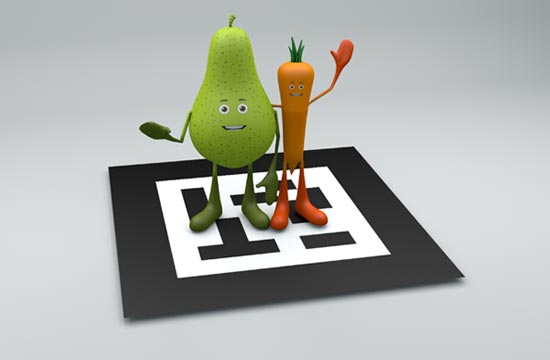
\includegraphics[width=.5\textwidth]{markerar}
				\caption{An example of how the marker technology works}
			\end{figure}
		
		\subsubsection{Location-based}
		
			Location-based AR mainly relies on GPS and many others spatial sensors (accelerometer, gyroscope, etc.), this technology is the milestone that let many developers produce AR games located in the real world.
			The main challenges for location-based applications had been the accuracy degree that was possible to achieve and the battery drain consequent to extended use of GPS; now the Google \lstinline|FusedLocationProviderApi| standardized the location retrieval exploiting together GPS, nearby Wi-Fi hotspots and cellular network while managing efficiently the requests to save battery charge; this allowed to reach 2-5 meters of accuracy. % MISSING SOURCE

		\subsubsection{Markerless Tracker}
			
			\begin{quoting}
				In its simplest form, tracking can be defined as the problem of estimating the trajectory of an object in the image plane as it moves around a scene. In other words, a tracker assigns consistent labels to the tracked objects in different frames of a video. Additionally, depending on the tracking domain, a tracker can also provide object-centric information, such as orientation, area, or shape of an object.~\cite{ylmaz:tracking}
			\end{quoting}
			
			This is the next generation of AR techniques. It uses particular algorithms to analyse the environment recorded from the camera and is capable of recognizing and tracking objects. Using this kind of technology, there is no more need to place any marker and the users can interact with the augmented world in a much more effective way.
			
	
	\section{AR In Mobile Devices}
	
		AR main target nowadays is of course mobile devices (both smart phones and smart goggles) given the simultaneous presence of a display, an embedded camera and more than decent processing units.
		
		This is pushing many companies in developing applications and frameworks, while a growing number of IT experts start to consider the AR more attractive than VR (Virtual Reality).
		
		The main limitation AR applications are facing in this field is surely the battery drain that CPU intensive tasks, GPS usage and enabled cellular network take within themselves, but those limits are being pushed further and further by new generation devices.
		
		Battery duration, as well as other tricks to limit power consumption (in this regard the new A10 processor from Apple, with power differentiated cores, is only the last of many optimizations), soon won't be a problem any more and AR applications will probably bloom on the market.
		
		\subsection{Main Frameworks}
			
			To build up the project, a AR framework with some specific features was needed, so the current panorama had been analysed to check which options had been developed in past years:
			
			\begin{description}
				\item[cost] free or with long enough free trial;
				\item[location-based] capable of managing \emph{at least} location-based AR;
				\item[licence] under MIT or Apache 2.0, looking forward to use the project with commercial purposes;
				\item[alive] with a strong and passionate community keeping the project alive;
				\item[documentation] good documentation by means of JavaDoc and examples;
				\item[2D] capable of showing \emph{at least} 2D pictures in the AR layer.
			\end{description}
			
			Unluckily, all those qualities could not be found in a single framework, in particular all free frameworks seems not to be alive any more.
			
			\subsubsection{Wikitude}
			
				By far, the best AR framework around. It manages 2D pictures and 3D animated objects, supports both native and JavaScript API, supports all 3 main AR technology (location-based, marker-based and markerless tracking); it is very active and always up to date with last OS and devices; it has a good documentation and is distributed for use in commercial projects.
				Only one point against: it is a subscription service and not really one of the cheapest.
				A free trial is distributed, but it puts a watermark when using the framework, so it was left out from the choice.
			
			\subsubsection{DroidAR}
				
				It supports marker-based and location-based AR; it has good documentation with JavaDoc wiki pages and examples; it manages both 2D and 3D objects.
				This seemed very promising at technical level, but had also a lot of flaws: the project has an open source GNU GPL v3 licence, which makes it impossible to use for commercial purposes as it is. Usage under another licence is possible, but paying a fee, so it is still not acceptable.
				In addition, the project on GitHub has been dead for 4 years now, because the maintainers switched to develop v2, which is closed source.
			
			\subsubsection{Mixare}
			
				Another open source project, another failure. Mixare can only manage 2D objects which consist in a picture or shape and an optional label. The documentation is really poor, and the location-based AR seems slow and buggy. It is free of charge, but only under GNU GPL v3 licence. Last but not least, the project has been dead for more than 4 years.
				Despite all those problems, the structure of the project and the ideas behind it are pretty clever, that is why it deserves at least a quote in this paper.
			
			\subsubsection{PanicAR}
			
				This framework seemed especially promising: it is focused on 2D pictures and location-based AR and it has a decent documentation.
				Unluckily, it is free of charge only for non commercial projects, otherwise a watermark is added; moreover the Android porting, the framework is iOs native, died 2 years ago.
			
			\subsubsection{BeyondAR}
			
				It has a really good documentation, tutorials and even a fully functional example application; it is location based and the API is pretty simple and intuitive; it is capable of managing both 2D and 3D objects. It is released under Apache 2.0 free of charge, still the development is open source.
				Unluckily the project had no further contribution for 2 years. Despite this fact, I decided to use it in the project, fixing by myself some known bugs and contributing to the development, hoping that the BeyondAR maintainer will come back at some point merging all the pull requests and resurrecting this already pretty good framework.
		
		\newpage
		
		\subsection{Main AR Games}
		\label{soa:games}
		
			Some pioneers already adventured in the mobile AR world and, considering the main product of this thesis is a AR application, it is important to briefly describe the ones who managed to have a decent success, either because they are relevant to show the level AR games reached today or because some of their mechanics and ideas are similar to the ones used in this project.
		
			\subsubsection{Pokemon GO}
			
				Developed by Niantic in collaboration with Game Freak, Nintendo and The Pokémon Company, it had been released to the public during 2016 summer and it quickly became a worldwide phenomenon, mostly because of the hype on the setting and, to a lesser extent, because of the actual technical advancements in AR technology it brings in itself, which in facts are scarce.
				Classifiable as an exergame (exercise game, fitness game) more than a Pokémon game, it heavily relies on location-based AR (there is just one feature that actually uses the device camera and it is usually turned off by users because it slows down the application and consumes more battery). It is based on a map where you can see your virtual alter ego and some POIs (Points Of Interest) with which you can interact in a very basic way.
				Three teams continuously fight one another to gain influence over special places and this pushes members of the same team to act in groups to claim the area ownership faster.
			
			\subsubsection{Ingress}
			
				Developed by Niantic (actually their first AR game), it is basically the same game as Pokémon GO, after you strip out the Pokémons and change the setting into a sci-fi one.
				The influence that this game had on Pokémon GO, both in terms of UX (User eXperience) and underlying technology, is pretty strong.
			
			\subsubsection{Life is Crime}
			
				Developed by Red Robot Labs, it is a location-based RPG (Role Play Game) with a criminal setting where your neighbourhood becomes the game board. The game is based on the concept of forming a gang with other players living nearby and make your reputation rise doing virtual crimes, trying to become the kingpin of your zone.
				The software house apparently shut down everything in 2015 after the use of bots and cheats ruined the game.
			
			\subsubsection{Zombie, run!}
			
				Developed by Six to Start and Naomi Alderman, it is the first and most famous exergame. Funded on Kickstarter, the game relies on location-based AR and is mainly focused on the single player experience together with a good background story, going bucking with respect to other AR games.
				The basic idea is to run away from zombies spawning near you and to listen registrations explaining the story, with sporadic events that brings the community together.
				The application has a seasonal life cycle where new missions, which means new background story pieces, are released in blocks of 30-40.
				A remarkable feature which had been added lets the users set an arrival point and generates a mission on-the-fly which will get them there.
			
			\subsubsection{Parallel Kingdom}
			
				Developed by PerBlue, it is the first location-based territorial RPG and is based, as many others, in conquering surrounding areas.
				The game is based on a map over which custom markers are placed to identify buildings, monsters and players.
				Both PvE (Player versus Environment) and PvP (Player versus Player) are supported, as well as travel, commerce and many features of classic RPGs.
				It is easily the most complete AR RPG on the market.
			
			\subsubsection{Father.IO}
			
				Developed by Proxy42, it is the first FPS (First Person Shooter) using AR techniques to become, as said by the funders, an “Augmented Reality Laser Tag”.
				It relies on a physical add-on put over the smart phone, called Interceptor, which is used to fire laser beams at other players and receive the ones coming from them.
				The interconnection system offers a good quality, since it combines GPS and local broadcasting to keep latency low and shots accuracy high.
				
	\section{Structured recreational events}
	
		In recent years, a particular kind of events entered the Italian panorama: these are usually transpositions of typical video-game adventures in real life.
		These events are characterized by organizers that pre-set a location (which can be a room or a city, depending by the nature of the event), ask a pretty high fee to participants, are limited in time and usually carry with them a concept of gaming different from the classical “playing for fun”: they usually present themselves as adventures and challenges more than games.
		
		\subsubsection{Room escape}
		
			\begin{quoting}
				An escape room is a physical adventure game in which players are locked in a room and have to use elements of the room to solve a series of puzzles and escape within a set time limit. The games are physical versions of “escape the room” video games. Games are set in a variety of fictional locations, such as prison cells, dungeons and space stations, and are popular as team building exercises.~\cite{wiki:escape}
			\end{quoting}
		
			This kind of game firstly spawned in 2006, then took over almost everywhere in the major cities of the world.
			It can be considered one of the first attempt of bringing something which has its place in a virtual reality, back to the real world: if not in the technical realization, it is analogous to the AR-based games in its fundamental principles.
		
		\subsubsection{Zombie Run}
		
			Following the idea of taking video-games scenario into life, this kind of events is based on simulating a survival horror setting, in which participants must usually run across a predefined path avoiding people disguised as zombies which will try to infect (touch) them. The path is fenced and traverses urban environment, giving to the event a pretty large playing area, even if limited.
		
		\subsubsection{Paint-ball / Soft-air}
			
			This is a transposition from actual warfare more than from video-games (which still helped in making it known to a larger public), but it has some interesting characteristics, like the extension of the area in which it is possible to play: for paint-ball it is roughly the size of a soccer field, but soft-air games can take place in a house (or group of houses) or even span over an entire forest.
	
	\chapter{Idea}

	The initial thesis goal was to produce a new AR framework but after some searches it became pretty much obvious that the current problem with this kind of framework is the inactivity rather than their shortage.
	So I switched to the production of an AR game, choosing an existing framework and updating/fixing it for my needs.
	
	\section{Serious Games}
	
		\begin{quoting}
			Games may be played seriously or casually. We are concerned with serious games in the sense that these games have an explicit and carefully thought-out educational purpose and are not intended to be played primarily for amusement. This does not mean that serious games are not, or should not be, entertaining.~\cite{abt:serious}
		\end{quoting}
	
		The first proposed idea was to build up a so called Serious Game, in particular an AR app that could serve as support to civil protection courses during their on-the-field simulations.
		The app structure closely resembled RTS (Real Time Strategy) games: one person, identified as a strategist, had a centralized control of the environment via a web app and could form groups of persons, identified as units each of which had a specified role, and assign those groups to a mission.
		Each role grant to the unit whom has it to perform one or more specific actions, while missions are no more than a sequence of predefined POIs to reach and actions to execute nearby those POIs.
		
		The idea was good, but after defining the basic game rules I preferred to switch to something more bound to the entertainment area, also because I did not had a direct contact with someone who could actually use and test the project after I had finished it.
	
	\section{Discworld - Ankh-Morpork}
	
		Searching for other ideas, I was suggested to chose an already existing board game and to transpose it's rules in an AR mobile game fashion.
		Excluding classic games, I focused on territorial control board games following the trend set up by Ingress and Pokémon GO.
		My choice fell on a game set in Terry Pratchett's Discworld setting, published by TreeFog Games with some particular attributes.
		
		The game setting is about a city in which the patrician just disappeared, leaving a power vacuum that different lords and prominent figures are willingly to fill.
		Two to four players represent the these personalities, everyone with a different victory goal, whom want to control the city.
		
		The game is turn based and controlled by cards which grant particular actions.
		Every player control his minions moving them around on the board (the city itself divided in neighbourhoods), assassinating enemy minions and building palaces to increase their control over certain areas (gaining power-ups).
		Build actions are possible only if the player has collected enough gold to pay taxes to do so, which can be collected with some cards or power-up.
	
		Every area chaos status is controlled by trouble markers that enable vicious actions, you cannot assassinate minions if the area is calm, and are modified by minions movements: every time a minion enter an area with other minions, a trouble marker is added, every time it exit, a trouble marker is removed.
		In addition, to bring in more suspense, a random event is fired every once in a while, creating havoc in everyone plans.
		
		Game mechanics below all this are in fact pretty simple and understandable, just reading the manual is enough and this is not usual for this kind of board games.
	
	\section{Game type}
	
		As we have seen in \autoref{soa:games}, nearly all of the currently widespread AR games are build up to be MMOG (Massive Multiplayer Online Games), based on the assumption that the user must be able to play whenever he wants and wherever he wants, in order to maximize the usage of the app and, indirectly, the revenue.
		The only analysed app that tries to offer a slightly different gaming paradigm is Father.IO which offer the feature to organize a laser tag, instead of just entering it on-the-fly when the user wants.
		
		While putting the user first is a legit choice, I wanted, for this project, to focus on another type of games.
		In fact, an aspect I wanted to keep while transitioning from a board game to an AR game was the idea that lays at the base of it.
		With Pokémon GO and the others, the idea is that when you does not have anything else to do, you play to escape boredom.
		With many boardgames (we are not talking of casual boardgames here), the idea is pretty much different: you decide to invest your time and spend efforts to organize a meet-up with person with or against which you want to compete.
		This kind of games stimulate your mind to think in a complex way and to be adaptive, instead of becoming dull while waiting for the next commitment of the day, and that is the same idea I wanted to put at the base of this project.
		
		Those kind of apps already exists, MoM (Mansion of Madness) for example will be shortly released with an associated app that will manage the board set-up and some part of the game previously managed by one of the players, and other boardgames publisher are following the same path.
		I got inspired by those news and decided to develop an app that could be an assistant to a board game, except that the board is this case is the real world.
		
		A concept has to be made clear: this kind of game is thought to be half-way between a Zombie Run and an organized evening event.
		The participation won't be for free and will be an all included package: dinner, game, possibly a prize for the winner.
		Given this, the registration will be done several weeks before the event take place and the participants will be strongly motivated to play and win (they spent for doing so), in this way we hope to keep away people not really motivated to play that could ruin the game experience.
	
	\section{Building up the team}
		
		As a programmer, there are some fields in a project like this app that I cannot do myself or that someone else can do better.
		Also, for personal aim, I never realize project that does not produce a result and that can be used in some way by others: it seems a waste to me.
		
		Following this principle, the obvious way to obtain an high level product was to compose a team that could overcome my deficiencies.
		The first thing I searched was someone to which I could hand the product once completed: it is possible to say that I wanted a problem to which my thesis was the solution.
		I found a good one into PassaPorta, an association active in Reggio Emilia which do entertainment both for kids and adults.
		In the latter case, it's mostly about thematic evenings, and this was exactly what I looking for.
		From PassaPorta I contacted Daniele Barozzi, who would help me in terms of how to manage an event with 20-25 people in play and which kind of limitations there would be in terms of game setting and mechanics.
		
		The second thing I needed was someone with a good knowledge in game design, in order to be sure that the game would be balanced and enjoyable and the rules would have been strong enough to resist to possible exploit tries.
		For this, more or less following the same idea that leads to hackers being employed in anti-virus companies, I contacted Valerio Catellani, a friend of mine, known for being the one who exploit the hidden mechanics of every game in order to win in an unexpected way. His job has been to help me transpose the board game mechanics to the AR app and stress test them in limit scenarios to be sure no one could cheat.
		
		Third, a graphic was requested, to help me defining the UX and to create beautiful images and UI for the game. Half my family helped me out for this: Francesca for general design definition and paper-based icons, Caterina for mock-up preparation and Luca for vectorial images.
		
		Last group of competence I lacked was the storytelling: a background story, established that we could not use Discworld setting because covered by copyright and we could not ask to the publisher because their permission to use that setting expired. Both Daniele Barozzi and my brother, Luca, helped me out in this, trying to write a background story that could fit the rules we previously defined and at the same time be appealing and coherent.
	
	\chapter{Design}

	My first aim, while starting the design part, was to produce a set of interfaces which could possibly support not only my particular game, but a various range of games which could base themselves on the same abstract logic.
	In particular, RTS AR games could be easily derived from the classes I produced for my project.
	Proceeding with the code writing I noticed that my aim was partially infeasible, for example in my try of generalize various type of games (Turn based, Checkpoint based, etc.) and location management, due to Java code rules and limitations in terms of Inheritance and Polymorphism.
	To overcome those limitations I would had to change the way my core interfaces worked, so I preferred to lower a bit the aim and to keep project-independent interfaces only for the really basic concepts.

	\section{Game Rules}
		
		Most of the rules of reference board game has been kept while translating the rules to the app; the most notably difference are the player management and the card system removal.
		
		\subsection{Leaders and Units}
		
			While in the original game we had 2-4 players, now we have 2-5 (and even more) teams, composed by 1 leader and 4-6 units each.
			The leader will represent the player of the original game, while units are the minions he would move; following this idea, the leader will be a strategist which will guide the units, like if he would be a player of an RTS game coordinating his units.
			More specifically, leaders of all the teams will be conduced in a room with a PC ready for every one and from there will be able to see everything that is going on in the board via a web-app: ally units, enemy units, their movements during the game, etc.
			The leader will be able to communicate to minions both in a textual or audio way, guiding them and telling them the enemy moves.
			They'll as well be the managers of the team gold reserve, lending money to units at the start of the turn, which will return into the team reserve at the end of the turn, if not used.
			Also a part of the role management will depend by leaders, as described below.
		
		\subsection{Board and Zones}\label{design:board}
		
			Board concept has been retained unchanged from the original game, but instead of a physical one in cardboard, a virtual one is generated on-the-fly starting from given centre and radius.
			The algorithm currently generate a pseudo-circular board with nine zones displaced in a symmetric way, with a central zone, 4 zones on the inner ring and 4 zones in the outer ring shifted by 45° with respect to the inner one.
			
			\begin{figure}
				\centering
				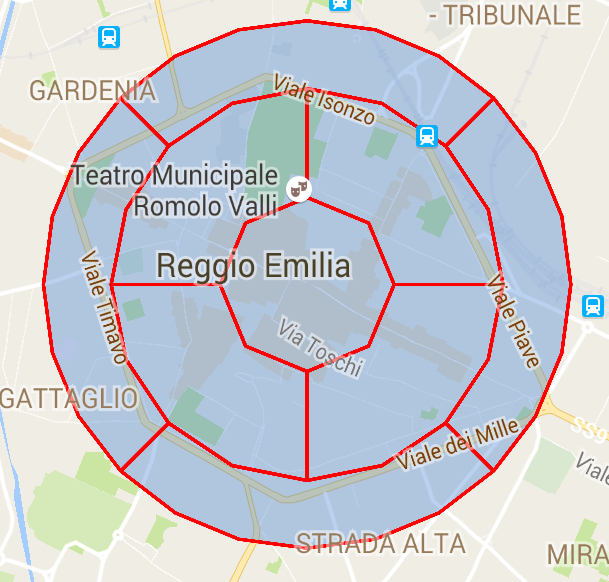
\includegraphics[width=.5\textwidth]{rightboard}
				\caption{Ideal shape of the board and zones}
			\end{figure}
			
			Zones all have the same area, thanks to a R simulation which calculated the right radius to use for different coordinates rings.
			Ideally, moving from a zone centre to another zone centre shall take 5 minutes and turn duration is related to this: the players shall make a choice between moving slightly (one zone or even staying in the same zone) and get plenty of time to perform their actions or move a lot (two or three zones) and running out of time to anything.
			Every zone grants a power-up when teams build on them (higher the building cost, more useful is the power-up) and the zones are randomly distributed on the board (eg. the power-up disposition will be unlikely to be repeated in subsequent games).
			Power-up activate at the begin of every turn.
			
			On a board of 9 zones, power-up are defined as in \autoref{powup:desc}, notice that some of them are referred to the role system, explained in the next subsection.
			
			\begin{table}
				\caption{Power-up description}
				\label{powup:desc}
				\centering
				\begin{tabular}{lccp{0.5\textwidth}}
					\toprule
					Name 			& Number 	& Cost 	& Description \\
					\midrule
					Money 			& 2 		& 4 	& Gain 3 coins \\
					Money 			& 2 		& 7 	& Gain 5 coins \\
					Calm 			& 1 		& 7 	& If the zone with power-up is chaotic, it is no more chaotic. Otherwise, calm a nearby chaotic zone, if more than one is present, it gets randomly chosen between the available ones \\
					Role 			& 2 		& 4 	& Gain one extra cop, assassin and builder role in your role pool \\
					Untouchable 	& 1 		& 9 	& You gain an untouchable bonus role: the player who get this cannot be killed \\
					Multitasking 	& 1 		& 9 	& You gain a multitasking bonus role: the player who get this can use both his actions for this turn \\
					\bottomrule
				\end{tabular}
			\end{table}
		
		\subsection{Roles and Actions}
		
			The card system had to be removed because, while easy to realize and use for single players, it would be too complex, time consuming and random based to use in a team-based game, especially if used through an app for mobile devices.
			But removing the card system come to a price, leaving a hole in the game mechanics behind himself: action assignment.
			To fill this hole, we prepared a new system based on roles, with the main objectives of creating a system which could let enough freedom of act to units, in order to remove the feeling of just being minions controlled by the leaders, and create a balanced game play.
			In this system only three main roles and a filler one, always available, can be used, everyone with it's actions and visibility rule particularities.
			In addition every role, except the filler one, must choose to perform an action between the two provided.
		
			\begin{description}
				\item[cops] can see their team mates and all assassins in the zone.
					\begin{description}
						\item[protect] all allies units within 10 meters to him cannot be killed.
						\item[calm down] following a path of randomly generated coordinates inside the current zone, the zone won't be chaotic any more.
					\end{description}
				\item[assassins] can see their team mates and all builders in the zone.
					\begin{description}
						\item[assassinate] if the zone is chaotic and he manage to stay within 10 meters to an enemy for at least 5 seconds, that enemy won't be able to use his action for the rest of the turn. If the assassinate unit owns money, the assassin rob it.
						\item[tear down] demolish a building, the owner team get refunded with half the price of the building and lose the zone power-up.
					\end{description}
				\item[builders] can see all other units in the zone, but does not know their role.
					\begin{description}
						\item[build] if the zone is not chaotic and the builder manage to stay near a randomly generated point in the zone for 2 min playing a small AR mini-game, a building owned by his team will rise there, provided he has enough money, and grant a power-up.
						\item[spread panic] following a path of randomly generated coordinates inside the current zone, it will become chaotic, if it was not already.
					\end{description}
				\item[collectors] can see only their team mates in the zone and money-grab points, but he knows the number of the other collectors in his same zone.
					\begin{description}
						\item[collect money] every time he reach a money-grab point, he earn one coin. Money-grab points are shared between all team and spawn in random locations on the board at the start of a every new turn.
					\end{description}
			\end{description}
			
			Roles has been defined to counter one other: cops can prevent the assassins to do their job, assassins are mainly equipped to attack builders and tear down what they made and builders hinder cops work by spreading the panic in a zone or trying to get the zone power-up.
			
			Some special roles, called bonus roles or enhancer roles, are earned as a consequence of particular power-ups, can be assigned by the leader to units, extra to the one usually distributed, and expires after one usage.
			Those roles change some in-game rules for the owners:
			\begin{description}
				\item[untouchable] the unit cannot be killed, either by assassins or events;
				\item[multitasking] the unit can perform both the actions of the primary role he chose.
			\end{description} 
			
			Role system is managed by leaders and units together.
			At game start, units own three roles (one per type) and leaders own six roles (two per type).
			During the start of each turn except the first, the leaders can give a role to every unit, taken from their role pool, and units will decide which role and associated actions will use for this turn.
			At the end of each turn every unit that used his action successfully will refund the spent role, which will be added to the leader role pool, ready to be redistributed on the subsequent phase; if the unit get assassinated or do not use the action he chose, the role will still be added to the leader pool, but on the subsequent turn.
			
			This system has been thought in order to give the leaders a way to "set the path" for his units, but still to let the units decide independently if they think that a different action will be more useful in that moment.
		
			% INSERT ROLE SYSTEM IMAGE HERE
			
			When giving out roles, leaders can also assign a mission to every unit which consist of a role, an action and a target (another unit or a zone).
			The unit can decide to accept the mission or to ignore it. If the unit decide to accept it, his role and actions are set automatically to the suggested ones and he'll see additional informations about his target (his positions, how many units are in the particular area, etc.) depending on the mission nature. If he accomplishes the mission, the team gain a small money bonus.
			
		\subsection{Starting zones}
			
			Various ideas had been evaluated to decide how the units should start.
			The main ones where: 
			
			\begin{enumerate}
				\item Following the original game, three fixed zones shall be the starting ones for every team, with the units equally distributed on them;
				\item All units start in the central zone;
				\item Units start from three fixed zones, but divided by team, instead of being equally distributed.
			\end{enumerate}
			
			The first option could be a problem in terms of organization, because every team start already divided and cannot make plans before the game start, thus bounding even more the units to instructions and suggestion given by the leader.
			But on another level, is the option that grant the more equilibrated start in terms of interaction between teams.
			
			The second one could seem funny at a first glance, but it will probably result in havoc and just a few of the units in game to actually succeed in their action for the first and second turn, slowing down the game.
			
			Third option has the exact opposite effect: for the first turns, teams will not interact at all or will do it very little and will only build on the zones near their starting zones or collecting money, thus crippling the game at the very beginning and giving a feeling of boredom. 
			
			Finally, the first option was selected for testing, even if the starting zones now are being randomly chosen instead of being fixed.
			% REVIEW, POWER-UP ARE STILL FIXED
			In fact, the main reason for which they where fixed in the first place, was that also the zones power-up where fixed: now that the power-up disposition is randomly generated, also the starting zone can be randomly chosen.
			
			All starting zones are set as chaotic by default.
		
		\subsection{Objectives}
			
			The objective system, which assigned a different one to every player, has been retained and most of the objectives are inspired to the ones of the board game. Leaders do not know which team has which objective (except his, obviously), but can deduce it from other teams actions and behaviour, since they will be informed of all objective in play, and try to hinder other teams.
			
			The objectives are defined as:
			\begin{description}
				\item[chaos] seven zones are chaotic;
				\item[peaceful] there are no chaotic zones or it's the eighth turn and nobody won;
				\item[omnipresent] there is at least one active unit (which has not been killed in the previous turn) or building on at least eight different zones;
				\item[control] the team controls (has more units+buildings on that zone of every other team) four zones;
				\item[rich] the team money reserve is at least of 50 coins (buildings add up to the money reserve as their's construction cost).
			\end{description}
			
			It's important to remind that objective accomplishment is checked at the very beginning of each turn: the team must keep the victory condition true until the current turn ends.
			
		\subsection{Random events}
			
			The random events effects did not change much from the original game, but of course their occurrence, which was bounded to the card system, had to be updated. Now the event occurrence is related to a certain probability which increase every turn in which no event take place, and reset to a minimum when one of them actually take place.
			
			The events are defined as:
			\begin{description}
				\item[a drake attack the city] extract a zone, all buildings in there are destroyed and all units currently there dies;
				\item[a fire breaks out] extract a zone, buildings in that zone are destroyed and another zone is extracted. If this new zone is nearby the previous one and contains buildings, the fire spreads and they are destroyed as well, then keep extracting a new zone until it stop spreading;
				\item[the fog falls on the city] visibility of each player toward others is blocked, both of team mates and enemies;
				\item[an explosion take place] extract a zone, buildings in that zone are destroyed;
				\item[time to pay taxes] every team must pay 3 coin for every building it owns or destroy it. Payment is done automatically in zone number order;
				\item[suddenly, earthquake] extract two zones, all building in there are destroyed;
				\item[a political disaster] extract a zone, since now the power-up of that zone is disabled for the entire match;
				\item[demons from below] extract five zones, a demon appears on each of those zones, more demons can appear in the same zone. As long as a demon is in it, the zone power-up is disabled, no coins are generated and it's not possible to build. Demons can be killed by assassins via an AR mini-game and have multiple lives.
			\end{description}
			
			Note that when is expressed that buildings are \emph{destroyed}, instead of demolished or tore down, it's meant that the owner team lose the power-up and get no refund; likewise, when is expressed that a unit \emph{dies}, instead of assassinated, it's meant that it lose all the money it was carrying and his role is automatically changed to collector.
			
			
		\subsection{Turns}
		
			The turn mechanics risked to be cut off the final version of the game, because it slowed down the game with respect to a much fluid and free system.
			In the end, we decided to keep it in order to synchronize the various phases (eg. money management, etc.) and avoid problems with the role system: the role refunding would not work in an environment in which all roles did not returned to the leader in the same moment to be distributed again.
			Every turn is divided in two sub-turns: leaders turn, which last 5 minutes and in which all the team management is concentrated, and units turn, which lasts 10-15 minutes and in which the real game take place.
			The basic idea is that leaders will have the 15 minutes of units' turn, while helping them, to define a strategy for next turns; in this way the 5 minutes of their turn are just to formalize and put in place the strategy previously defined.
			
			This is obviously needed also to prevent units from staying still for too much time, which would lead to boredom and ruin the perpetual tension feeling we wanted to grant them.
			
	\section{Variations}
		
		Considering the high team coordination needed to play a game like the one described above, some variations had been prepared to simplify the game and address some mechanics which can be too hard to get for a new player.
		In particular, the fact that leaders do not physically take action in the game could be a problem for various reasons:
		
		\begin{itemize}
			\item a good preparation and knowledge of the game rules is needed to be able to lead the team to victory, which can be hard to achieve in events like the one proposed, because leaders would have only a few hours to prepare: definitely not enough;
			\item while staying in a closed room being the mastermind of your group is could be an interesting idea for someone, there's a possibility that leaders will instead feel isolated and not actively participating to the game;
			\item leader participation would require a web-app development and deployment in order to test also the units part, but this thesis is about the mobile application and the game in itself: this could only slow down the production;
			\item while an app entirely running on smart phone does not require to provide any hardware (everybody have one these days), to use a web app we would need to set up 4-5 computer.
		\end{itemize}
		
		\subsection{Limited leaders}
		
			One possible way to address those problems is reducing leader's duties in the game, removing the web-app necessity and integrating team management in the app.
			In this scenario, leaders plays with their team as they were mere units choosing a role and an action, lose the vision of everything (they only see their team units position) and in general they now look more alike to an on-the-field sergeant or a super-unit than an high level strategist.
			They keep managing the team money reserve and role assignment, but from now on the role pool will be smaller and the system simpler, there won't be missions, for example.
			
			This resolve most of the issues: leaders are now playing with others team members and are generally more involved in the game, no web-app is needed (and thus no computers) and they does not need an in-depth knowledge of the game rules, because they are required only to manage money and a simplified role system.
		
		\subsection{No leaders}
		
			The natural evolution is to remove the leader character at all.
			Here, teams are formed by peer units which together decide where before was leader duty to do so, helped by the app to do so.
			When the team cannot get to a shared decision, the system will follow a default path or choosing randomly between the options, usually resulting a disadvantage to some of the units or to the entire team: this shall convince the team to collaborate in a positive way.
			
			\textbf{The project will implement this variation of the game.}
			
			% FIXED ROLE POOL?
			\subsubsection{Roles}
			\label{nolead:role}
				Role distribution in this scenario change drastically: role pool is fixed (two roles per type, infinite for the filler role) and the role choice is bounded to a timer.
				Every unit must select his preferred role for that turn, if there are left of that kind, and communicate with the team to resolve possible conflicts (eg. three units want to be assassins).
				When the timer stops, every unit get the role he selected and must choose the action. Conflicts are avoided in a first-come, first-served fashion.
				
				Bonus roles are managed more or less in the same way: players can ask to use one of them \emph{in addition} to their preferred role, and conflicts are avoided in the same way as the normal roles.
							
			\subsubsection{Money}
			\label{nolead:money}
				Money distribution is managed similarly: when the turn starts units ask to borrow a certain amount of money from the team reserve, if there is enough money for everyone the money is simply distributed to who asked for them, while if the requested money exceeds the team reserve, units must discuss between them to resolve possible conflicts.
				When the turn ends, money from all units is put back into the team reserve.
				
				This could also be achieved by an on-the-fly request only when the money is needed, but this alternative could bring to even more problems: the rule that allowed assassin to rob his victim partially break apart in this way, because only the collectors (or another assassin which had previously killed a collector) will have money with them, and the loan will probably need a confirmation vote from all others units, wasting a lot of time.
		
	
	\chapter{Implementation}

	\section{Infrastructure}
		
		\subsubsection{Team management}
		
			Considering the kind of event bounded to the game usage, something gets clearly on mind: the team registration must be done long \emph{before} the event.
			
			For this, a simple website needs to be developed, in which teams must be able to enrol for events, specifying the emails of all team members and a reference person which will take care of the team management (eg. player removal or substitution).
			In this way organizers will be able to directly communicate with all players of a given event.
			This project won't cover that part and focus only on the mobile application part.
		
		\subsubsection{Data storage and manipulation}
			
			Instead of relying on an old-style SQL database accessed from a PHP/Java environment, the data management is achieved using a new platform: Firebase.
			This service does a great job keeping data in sync between heterogeneous devices and offers a powerful API, together with a solid yet flexible security system based on data access rules.
			One drawback is that complex queries cannot be performed with a single request and must be done using nested calls to the database, even if the heavy optimization implemented mitigate this problem.
		
		\subsubsection{Game}
		
			Being backed by Firebase, the first idea was to avoid the back-end server completely, implementing some sort of all-in-app distributed game logic.
			Unluckily, it resulted obvious that game status and phases, together with some conditions checks, needed a centralized code to be managed easily.
			Actually this constraint is more a design-driven choice than a mandatory one: all the game logic \emph{could} be realized directly on the mobile application, synchronizing between all devices, but this would result in messy code and possibly open some security issues: not the most desirable scenario at all.
			Considering this, the KISS (Keep It Simple, Stupid) approach has been followed and the two aspects of the game were separated.
			
			\paragraph{Game logic}
			
				To support the game logic, a Java task on the server will run in loop interacting with the real time database observing the actions made by the players and eventually acting on his own to modify the game internal status. In particular it takes care of:
				\begin{itemize}
					\item \textbf{initialization:} preparatory steps to execute before a match takes place (initial status, board set-up);
					\item \textbf{phases:} manages phase changes and the timers associated with them;
					\item \textbf{objectives:} check every turn if a team reached his objective;
					\item \textbf{events:} manages the probability of an event to take place, its random selection between the available ones and applies its effects;
					\item \textbf{status reset:} every temporary status change (zones power-ups and events effects) is reset to its original value at the end of turn;
					\item \textbf{power-up:} applies effects of the power-ups;
					\item \textbf{log:} record all match actions and events in order to enable post-match studies and replays.  
				\end{itemize}
				
				The many timers that the game logic must share with the application are saved on the database as their expiration date. In this way it's possible to every device in any moment to calculate the missing time to the expiration and set an internal time-out on their own.
			
			\paragraph{Players logic}
			
				Player logic, instead, is managed by the application running on every device, which communicates directly with the real time database. In particular it takes care of:
				\begin{itemize}
					\item \textbf{messenger:} a dedicated messenger will be provided to allow in-game communication between team members;
					\item \textbf{localization:} keeps track of players last known position and last time they were active;
					\item \textbf{roles:} the role and action selection system will be entirely implemented by the application, the server will only observe those operations;
					\item \textbf{board visibility:} which part of the board, which players and which markers show to each player will be decided by the application, depending on the role and location of current player.
				\end{itemize}
			
	\section{Work flow}
	\label{workflow:general}
		
		The game follow a sequence of statuses, one of which is turn based (the more important, the actual "gaming" part).
	
		\subsubsection{Inactive}
		
			The match has not been initialized, it's the default value when there is no game available.
	
		\subsubsection{Initialize}
		
			The match is being initialized, performing various steps following a particular order:
			
			\begin{enumerate}
				\item The board centre and radius are fetched from the database;
				\item Clean all data from previous match, in particular the random event probability and the turn counter are set to 0;
				\item Instantiate random events and reset them as eligible to be drawn;
				\item Instantiate zones;
				\item Generate the board;
				\item Load zones info (centre coordinates, perimeter points, cost, description, etc.) and status (initially calm) into the database;
				\item Randomly chose the starting zones, setting them as chaotic;
				\item Retrieve teams and units from the database;
				\item For every team: 
				\begin{enumerate}					
					\item For every member of the team:
					\begin{enumerate}
						\item Select the starting zone with fewer units already assigned to it;
						\item Assign the unit to that starting zone;
						\item Set unit starting position to the centre of that zone, reset his last position and last on-line values, set him as not ready to start the game;
						\item Increase the counter that keeps track of the users which must reach their starting position;
					\end{enumerate}
					\item Randomly chose an available objective and assign it to the team;
					\item Set the initial team's money reserve;
					\item Set the initial team's role pool.
				\end{enumerate}
			\end{enumerate}
		
		\subsubsection{Prepare}
		
			Units must reach their starting position: once everyone is within 10 meters from it, all listeners on the database are initialized and the match starts.
		
		\subsubsection{Start}
		\label{workflow:start}
			
			This is the core of the game: it's a loop which every turn execute five logical phases.
				
			\paragraph{Control}
			
				Here the turn preparation is done: this part does not directly interact with the users, mostly checks and status updates are performed.
			
				The first check is on the victory criteria: all teams' objective is checked against the current game status. If one of them is fulfilled, the games ends.
				
				Then, as first operation of the new turn, the turn counter is increased, its value is updated on the database and all temporary conditions are reset to their original values.
				
				The second check is on the random event: if there is at least one available event to fire out, a randomly generated percentage number is tested against the current event probability and, if it's lesser or equal, the event is fired and the event probability is reset to the minimum value.
				In case the probability is set to 0.00 (possible only if it's the first turn), it is instead set to the minimum value and the test is skipped.
				
				Lastly, the power-ups gained by the zones on which a building have been constructed are applied.
				
			\paragraph{Roles}
			
				Here the roles selection system is activated and players will choose their role for that turn following the rules explained in \autoref{nolead:role}.
				The server will manage the timer of four minutes.
				
			\paragraph{Actions}
				
				After the role selection, another timer, one minute long, is set to let the players choose their action.
				
			\paragraph{Money}
				
				Lastly, the money are borrowed by the players from team reserve as explained in \autoref{nolead:money}.
				This phase also last one minute.
							
			\paragraph{Turn}
			
				Here the real game takes place: the server will keep a timer of fifteen minutes during which the players can act following their team objective or disrupting others plans.
				Every action will be performed by the application, communicating directly to the database without server interaction. This does not mean that it will stay idle: every action made, as well as every player movement, will be recorded by the server on a log file from which will then be possible to run a match replay, in order to get statistics and to study it.
			
		\subsubsection{End}
		
			All players are notified that the game ended, displaying the winner team name, then a gathering location is shown and all players must reach it in order to meet-up with organizers and continue the event: the winner team will likely be awarded at this point with the possible prize.
			
	\section{Data model}	
		
		Data are modelled both on Firebase with his internal rules and in Android/Java with classic Java interfaces/classes.
		Android model is a simplified version of the Java one, with many fields which are changed from custom classes to simple strings, because the clients only need a subset of the operations needed by the server and cannot access all informations (many are restricted based on who's reading them).
		
		\subsection{Firebase}
			
			In Firebase there is no concept of "data model" and the data structure definition de facto relies on the powerful yet flexible rule system which manage data access and manipulation.
			The rule system allows to validate incoming data with a JavaScript-like language encapsulated in a JSON and to define constraints, for examples, on which children a particular branch must have in order to be valid. This can be seen as defining a constructor in Java which enforce the initialization of mandatory fields.
			
			Considering that some lines are pretty much the same over various rule definitions, some kind of legend can be useful to cover the more common ones.
			
			\begin{itemize}
				\item \lstinline|".write" : false| \\ when no \lstinline|.write| rule is defined, this one is assumed for that level, because \lstinline|.write| rule defaults to \lstinline|false| when not specified;
				\item \lstinline|".validate" : "newData.hasChildren(['field1', 'field2', ...])"| \\ if this branch is defined, then the specified fields inside it must exist as well;
				\item \lstinline|"$var" : { ... }| \\ a wild-card who goes one level deeper in the branch keeping a reference to the key in which we are in, it can be used as a variable inside that scope rules. For example, in a branch \lstinline|dinosaur| with a collection of dinosaurs by name, \lstinline|$dino| will contain the name of the dinosaur of the branch we are in;
				\item \lstinline|{ ..., ..., "$other" : { ".validate" : false } }| \\ any field different from the ones specified is not allowed.
			\end{itemize}
			
			Firebase model is obviously simpler and looser than it's Java counterpart and has at top level only four branches.
			
			
			\subsubsection{Game}
			
				\lstinputlisting[caption=Game branch rules,
								firstline=3,
								lastline=66]{main/listings/firebase.json}
				
				All data needed to manage a game instance are contained here.
				Everybody can read at this location, but no one (except the server service account) has write permission, as shown by line~\ref{firebase:game:read} and the absence of the \lstinline|.write| rule. \\
				
				\paragraph{status - line~\ref{firebase:game:status}}
				Represent the status in which the game can be, as seen in \autoref{workflow:general}, plus \emph{PAUSE} and \emph{RESUME}.
				His Java counterpart is an enumeration class, and his content \emph{must} reflect the literal representation of that enumeration.
				This is used by the application and the server to check in which status the game is, considering that both are designed to take into account crashes and disconnection resuming where the game was left as soon as they reconnect.
				Some application components, like the one which display the users on the map as described in \autoref{focus:map}, even use this information to alter their internal status and change their appearance.
				
				\paragraph{board - line~\ref{firebase:game:board}}
				Used mostly during \emph{INITIALIZE} operations to generate the game board, see \autoref{focus:board}.
				Contains the centre and radius of the board itself.
				
				\paragraph{unitsToWait - line~\ref{firebase:game:wait}}
				Used during \emph{PREPARE} to keep track of how many units have yet to reach their starting position.
				It's initialized with the total number of players during \emph{INITIALIZE} and decremented by 1 every time a unit reach his starting position.
				Instead, if a unit who already reached it move away, the counter is increased by 1.
				When it reaches 0, the server updates game status to \emph{START} and all clients (who previously set a listener on it), will move from prepare activity to game activity.
				
				\paragraph{phase - line~\ref{firebase:game:phase}}
				Works in the same way, and with similar use cases, to the status field.
				Keeps track of the current phase while in \emph{START}, as seen in \autoref{workflow:start}.
				
				\paragraph{timer - line~\ref{firebase:game:timer}}
				Used during \emph{START}, is the moment in which the currently active timer will expire. It's updated by the server service account each time a new timer is set and read by all clients devices to synchronize with the game workflow.
				
				\paragraph{turn - line~\ref{firebase:game:turn}}
				Used during \emph{START}, is the turn counter. Considering the game structure, which can potentially go on forever until a team wins, this could seem useless, but to avoid exactly this scenario one objective has been designed to cut the game after 8 turns.
				This countermeasure has been taken to address multiple constraints, mainly battery drain, game pressure and players concentration.
				
				\subparagraph{battery drain}
				Mobile games always find a fierce opponent in battery drain, just by considering that the screen must always be on while playing.
				In this case, the problem is even more accentuated, given that the game requires not only the screen to be turned on, but also GPS, internet connection and, while in augmented reality mode, even the camera steadily capturing and processing images.
				A single turn is composed by 20 minutes, asking the battery to support all this consumption by his own for a total of 140-160 minutes is pretty unrealistic, unless all players got an high end smart-phone.
				Another way to address the problem could be to give each player a power bank and an USB cable, which will be a fall-back in case 8 turns will prove themselves to be too short for other teams to compete.
				
				\subparagraph{game pressure}
				Most games are played to relieve stress. This is not the case. In fact, this game is based on principles typical of competitive games and pressure over the players must stay high during all the match. Removing the turn limit could lead some people to relax and not taking the game seriously, ruining the game both for their opponents and teammates.
				Unlimited play time also let users correct their mistakes, because a strategy defect in a turn can be fixed during the following 3-4 turns while keeping on with the team objective: this again make the game longer and does not punish enough who make mistakes, leading to a game where taking a risk has few to no consequences.
				There will be plenty of time to relax before and after the game, but \emph{during} the game, pressure must stay high.
				
				\subparagraph{players concentration}
				As a student and worker, I know that human concentration has limits. The game structure based on 5 minutes of decision making followed by 15 of running around and doing stuff has been thought taking this into consideration, but it's impossible to stay steadily concentrated on something for more than two hours.
				To ensure players fun, the game must be as short as possible, or they will quickly get bored and tired.
				
				
				\paragraph{event - line~\ref{firebase:game:event}}
				Used during \emph{START}, keeps track of the event probability and of which events didn't happened yet (every event may take place only one time per match). This info could be, and actually is, stored directly in the server, but it's copied and kept up-to-date also on Firebase in order to prevent data loss upon server crash. Moreover, putting it here, we can let the players know which events can still happen.
				
				\paragraph{winner - line~\ref{firebase:game:winner}}
				Used during \emph{END}, it's the id of the team that won the game.
			
			\subsubsection{Team}
			
				\lstinputlisting[caption=Team branch rules,
								firstline=68,
								lastline=132]{main/listings/firebase.json}
				
				Information about teams is stored here.
				Everybody can read at this location, but no one (except the server service account) has write permission, as shown by line~\ref{firebase:team:read} and the absence of the \lstinline|.write| rule.
				The \lstinline|.read| command had to be moved out of the single team scope, otherwise units would be able to read every single team branch, but not the whole list. \\
			
			
				\paragraph{color - line~\ref{firebase:team:color}}
				The color associated with this team. Considering that there could be the necessity of displaying units of different teams all together on the board (both in the map and in the AR part), a random color chosen between the predefined ones is assigned to every team during the team registration. This color will be used every time there will be the necessity to show that an unit is of a particular team or to show the team generic information.
				It's stored like a color name, instead of an hex code, in order to directly use the \lstinline|Color.valueOf(name)| method present on Android (otherwise we would have to use the \lstinline|ResourceCompat| support class to get it and the code would have been less human-readable); this could be changed if a more specific color selection is needed.
			
				\paragraph{name - line~\ref{firebase:team:name}}
				Specified during the team registration, it will be displayed to identify the team when required.
				
				\paragraph{objective - line~\ref{firebase:team:objective}}
				Randomly assigned during the game initialization, describes the victory criteria of the team.
			
				\paragraph{members - line~\ref{firebase:team:members}}
				All members of the team are listed within this branch, with the units keys as the sub-branch keys and value set to \lstinline|true|. This is an easy way to access the information from validation rules of other fields: checking if the branch \lstinline|team/<team_id>/members/<unit_id>| exists is the easier way to know if an unit is a member of a particular team.
			
				\paragraph{money - line~\ref{firebase:team:money}}
				Money reserve of the team. Both \lstinline|loan| and \lstinline|maximum| fields must always be set. At the start of the game \lstinline|loan| is initialized to 0 and \lstinline|maximum| to 10 coins.
				The money management works as explained in \autoref{nolead:money}.
				
				\lstinline|maximum| decreases accordingly to the loan given in \emph{MONEY} phase, so players from other teams can check how many coins have been given to units comparing the reserve before and after that phase, and increases again during the \emph{CONTROL} phase in which money from every unit flows back to the team reserve.
				When assassins demolish buildings of this team, half the price paid to construct them is refunded and therefore added to this field.
				
				\lstinline|loan|, instead, keeps track of the loan requested during \emph{MONEY} phase and must be comprised between 0 and the maximum money in the reserve. This is one of the few fields which are modifiable by units inside the team branch, but can be touched only by team members.
				
				\paragraph{roles - line~\ref{firebase:team:roles}}
				Role pool data. Both \lstinline|current| and \lstinline|maximum| fields must always be set. At the start of the game both \lstinline|maximum| and \lstinline|current| fields are set to the initial role pool: 2 cops, 2 assassins, 2 builders, 999 collectors, 0 untouchable and 0 multitasking.
				The role management works as explained in \autoref{nolead:role}.
				
				\lstinline|maximum| field is updated at the end of \emph{CONTROL} phase of every turn, after taking into account possible random events and zones power-up.
				
				At the very beginning of the \emph{ROLE} phase, \lstinline|current| child values are reset to be equal to the \lstinline|maximum| ones, then they're updated every time a unit chooses his role or changes his already chosen role. In this way, other units can easily see which roles are still available for them to choose.
				Those values cannot ever be negative and can be at maximum as much as their counterparts in \lstinline|maximum| field.
				This is one of the few fields which are modifiable by units inside the team branch, but can be touched only by team members.
			
			\subsubsection{Unit}
			
				\lstinputlisting[caption=Unit branch rules,
								firstline=134,
								lastline=195]{main/listings/firebase.json}
			
				Information about units are stored here.
				Everybody can read at this location, but only the unit itself (and the server service account) has write permission, as shown by line~\ref{firebase:unit:read} and~\ref{firebase:unit:write}.
				The \lstinline|.read| command had to be moved out of the single unit scope, otherwise other units would be able to read every single unit branch, but not the whole list. \\
			
				\paragraph{username - line~\ref{firebase:unit:username}}
				Unit username, as inserted during the registration. It's used to identify the unit in many different scenarios: on the map fragment, in AR activity, in the team management fragment, etc. Not to be confused with the email, needed for the login and saved together with the password in the Firebase Auth system.
			
				\paragraph{team - line~\ref{firebase:unit:team}}
				Reference to the team of which this unit is member. It's a redundancy, we could check every team if this user is present in the \lstinline|members|) field, but in Firebase this is normal, considering the difficulty and limitation in query system.
				It's validated to be sure that the inserted identifier actually reference an existing team.
			
				\paragraph{lastOnline - line~\ref{firebase:unit:online}}
				If the unit is not currently on-line (see \autoref{model:presence}), this value represent the last moment in which he was seen on-line. This is used mostly by the game logger (\autoref{focus:log}) or to display how much time passed since a unit accessed the application. It's updated when the unit disconnect from the system, as explained in \autoref{focus:presence}.
				
				\paragraph{lastPosition - line~\ref{firebase:unit:lastpos}}
				The last GPS position in which the unit was seen. AR parts of the project are based on this field (and it's updates from all units) to show where other units are.
			
				\paragraph{zone - line~\ref{firebase:unit:zone}}
				The last zone in which the unit was seen. It's updated when the unit move out of his previous zone for at least 10 meters. This field is the main component of the visibility rule system used on the map, as described in \autoref{focus:map:visibility}. It can assume a value from 0 to 9, where 0 means that the unit is currently out of the board, while 1 to 9 represents the zones with that number as key.
				
				\paragraph{startPosition - line~\ref{firebase:unit:startpos}}
				Used in \emph{PREPARE}, is the GPS position of the starting point of the unit. It's set in \emph{INITIALIZE} where units are equally distributed on 3 randomly chosen starting zones, and correspond to the zone centroid.
				When the user reaches his starting point, it's asked to stay near it until all other units has reached theirs. He can move as far as 20 meters from it, if he goes further, the application will notice and ask him to return to the starting point.
				
				\paragraph{ready - line~\ref{firebase:unit:ready}}
				Used in \emph{PREPARE}, record if the unit reached or not the starting point. Based on this field, we are able to distinguish from a unit which arrived to the starting point and then moved slightly away and someone which arrived near the starting point but never reached it for real, still resulting not ready to start the game. Every time a new unit sets this field value to \lstinline|true|, he will also decrease by one the \lstinline|unitsToWait| field on the game branch.
				If the unit moves too far away from the starting point, the value is reset to \lstinline|false| and \lstinline|unitsToWait| will be increased by 1. 
				
				\paragraph{role - line~\ref{firebase:unit:role}}
				Used in \emph{START}, represents the current role of this unit. By default it's set as \emph{UNSPECIFIED}, value to which is reset at every \emph{CONTROL} phase.
				During \emph{ROLE} phase, may change several time while team members decide who'll take which role, then it cannot be modified until next \emph{ROLE} phase.
				The chosen role also impacts on the actions which can be selected by this unit in the subsequent phase, \emph{ACTION} one.
				This field is one cornerstone of the game, because greatly influence visibility rules and interactions between units.
				
				\paragraph{action - line~\ref{firebase:unit:action}}
				Used in \emph{START}, stores the chosen action. It's updated in \emph{ACTION} phase and, while not influencing the visibility rules like the \lstinline|role| field, defines at a more fine level the interaction with other units. Usually every role grants access to the choice between 2 actions, except from the \emph{COLLECTOR} role which grants just one action. Using the \emph{MULTITASKING} power-up it's possible to select both the actions provided with every role, but this feature has not been modelled yet, it will probably require to change the \emph{action} field type from \emph{String} to \emph{List}.
				
				\paragraph{money - line~\ref{firebase:unit:money}}
				Used in \emph{START}, this field is used, in different phases, to record either the coins the unit ask to borrow from team reserve or the coins he's carrying with him. It's possible to get money in 3 ways:
				\begin{description}
					\item[asking a loan] as described in \autoref{nolead:money}, in \emph{MONEY} phase;
					\item[collecting coins] if the \emph{COLLECTOR} role has been chosen, using AR to find and pick up coins, in \emph{TURN} phase;
					\item[robbing other units] if the \emph{ASSASSIN} role has been chosen, assassinating someone which is carrying coins, in \emph{TURN} phase.
				\end{description}
			
				Money can be used by builders to construct buildings which cost differs from zone to zone, depending on the power-up usefulness.
			
			\subsubsection{Zone}
			
				\lstinputlisting[caption=Zone branch rules,
								firstline=197,
								lastline=280]{main/listings/firebase.json}
								
				Information about board zones is stored here.
				Everybody can read at this location, but no one (except from the server service account) has write permission, as shown by line~\ref{firebase:zone:read} and the absence of the \lstinline|.write| rule.
				The \lstinline|.read| command had to be moved out of the single zone scope, otherwise other units would be able to read every single zone branch, but not the whole list.
				It must be noted that zone identifier must be an integer between 1 and 9, in order to make the \lstinline|near| field work correctly. \\
				
				\paragraph{description - line~\ref{firebase:zone:description}}
				Zone description, which is usually related to the power-up effect.
				
				\paragraph{cost - line~\ref{firebase:zone:cost}}
				Coins which must be paid to construct a building on this zone. To be able to do so, builders must carry with them at least this amount of coins. Upon a building demolition, half the cost is refunded to the owner team. Upon constructing a building, instead, the team gain the zone power-up, taking it from the previous possessor, if any.
				
				\paragraph{center - line~\ref{firebase:zone:center}}
				GPS position of the centre of this zone. It's used in \emph{PREPARE} as starting point for units.
				
				\paragraph{perimeter - line~\ref{firebase:zone:perimeter}}
				Collection of GPS position of all vertex composing the zone perimeter. It's set for the first and only time in \emph{INITIALIZE} and used to print the game board on the map and to check if a unit is in this zone or not. It's important to note that vertexes must be ordered, otherwise the perimeter would result a useless scribble on the map.
				
				\paragraph{near - line~\ref{firebase:zone:near}}
				Collection of zones near to this one, needed to execute some power-up effects.
				The added values are checked to be actually reference to other zones.
				
				\paragraph{chaotic - line~\ref{firebase:zone:chaotic}}
				The status of this zone: \lstinline|true| if chaotic, \lstinline|false| if calm. Builders cannot construct in a chaotic zone, while assassins cannot assassinate in a calm zone. This field can be updated only by the units which chose \emph{CALM} or \emph{PANIC} actions in this turn.
				
				\paragraph{controller - line~\ref{firebase:zone:controller}}
				Team which holds control on this zone. The control mechanic is needed for an objective, which requires to gain control of 4 zones to win the game. A team is called "controller" of a zone if the sum of his buildings and units in it is higher than the one of every other team. This mechanic is better explained in \autoref{focus:control}.
				
				\paragraph{units - line~\ref{firebase:zone:units}}
				List of units currently in this zone, it's used to check which teams control this zone and only the units themselves can add/remove their child branches at this path. Of course, they must be valid and authenticated units.
				
				\paragraph{buildings - line~\ref{firebase:zone:buildings}}
				List of buildings constructed in this zone. Every building must have a \lstinline|owner| field which stores his owner team id. Only units which chose \emph{BUILD} or \emph{DEMOLISH} action for this turn can update data at this location (constructing or demolishing a building).
			
			\subsubsection{Presence}\label{model:presence}
		
				\lstinputlisting[caption=Presence branch rules,
								firstline=282,
								lastline=294]{main/listings/firebase.json}
									
				This branch support the presence management system, which is discussed in more detail in \autoref{focus:presence}.
				Everybody can read at this location, every unit can write here as well, but only in the sub-branch based on his id, as shown by line~\ref{firebase:presence:read} and~\ref{firebase:presence:write}.
				The \lstinline|.read| command had to be moved out of the single unit scope, otherwise units would be able to read every single unit branch, but not the whole list.
				The only value which every unit branch can assume is \lstinline|true|, which states that unit is currently on-line. Conversely, if the branch with the given unit id doesn't exists, the unit is off-line.
			
		\subsection{Java/Android}
			
			The Java data model reflects the Firebase data structure and the Android one is a copy/paste but with a lot of simplifications. Since it's not interesting to explain extensively all its classes with fields and methods, only notable pieces of code (the few which will not be covered in \autoref{focus:general}) and differences between Java and Android models, and why they exists, will be described.
			
			Obviously, the \lstinline|FirebaseSync| interface, as described in \autoref{focus:log}, is implemented only on the Java data model and not present in the Android one.
			
			\subsubsection{Game}
		
				This is the most important class of the server data model because it's the actual endpoint \emph{and} the game abstraction: in a multi-game environment it should only be the game abstraction, but for testing purposes with only one game at a time, the two functionalities have been combined in a single class.
				
				The static \lstinline|main| method is defined here and performs the endpoint operations:
				\begin{description}
					\item[Firebase service account] The server must be able to update the database ignoring some rules, as it's possible via the dashboard. Firebase permits to activate a service account with this power, based on a login JSON token previously downloaded and included in the project.
					\item[Initialization] For testing purposes, only 4 users are actually registered on Firebase with a real mail and data, all others are dummy records. This part resets the root branch setting it to null value, then proceeds in filling it again with all the values needed for a match in \emph{INACTIVE} status: board centre and radius, teams and units dummy records, etc.
					\item[Launch the game instance] The game instance, which implements the \lstinline|Runnable| interface, is eventually launched on a new thread, providing the Firebase reference initialized before.
				\end{description}
				
				The \lstinline|run| method called when the thread is started just adds a listener on the game \lstinline|status| field: every time it gets an update, a private method corresponding to the new status is called and acts as described in \autoref{workflow:general}.
				It's important to note that only the server itself can change the \lstinline|status| field, the Android clients cannot access that branch in write mode.
				
				All match-related tunable parameters are defined here, like:
				\begin{itemize}
					\item Number of starting zones;
					\item Initial money for every team;
					\item Duration of the various phases;
					\item Zones tuning parameters;
					\item Objectives tuning parameters.
				\end{itemize}
			
				Literally every information present in the Firebase Realtime Database can be accessed in some way from this class, in particular it keeps references to:
				\begin{itemize}
					\item The turn counter;
					\item Event list and probability;
					\item Board object;
					\item Teams and units lists;
					\item Temporary match-affecting statuses (eg. fog status which limit visibility for one turn).
				\end{itemize}
			
				In Android, this class is not present.
				
			\subsubsection{Team and Objective}
			
				The members management (add, remove, get) has been stripped out in the Android version of the \lstinline|BaseGroup| (of which the actual \lstinline|Team| class is an extension) because not needed, all teammates are treated like normal units and their team id is enough to identify them. 
				
				The team color is represented as a string in Java, where it must only be stored as in Firebase Database, but becomes an integer on Android, where it's used via the \lstinline|Color| native class (not present in Java), changing also its getter/setter to manipulate the alpha value of retrieved color.
				
				While in the Java version the objective field of \lstinline|Team| is represented as a reference to an instance of \lstinline|BaseObjective|, needed to check victory criteria and store the objective description, on Android it's simply a string containing directly the team objective description, so the \lstinline|BaseObjective| class and its derivatives have been removed.
			
			\subsubsection{Unit}
			
				This central class of the Java model is not present in the Android version, because all pieces of code which required to store information about the units (teammates data using Firebase UI and players data storage in \lstinline|GeoFragment| module), also needed an ad-hoc implementation too different from the server one and have instead been done as inner classes.
			
			\subsubsection{Zone and Board}
			
				These classes have been removed from the Android data model because similar classes from the Google Maps SDK already provided the same pieces of information, while adding some useful methods, apart from being mandatory in order to use most of the utilities in the library.
				
				The only interesting feature in the \lstinline|BaseZone| class is the zone control system, which will be explained in \autoref{focus:control}, and is not needed on the Android counterpart.
			
			\subsubsection{Role and Action}
			
				Those classes have been retained the same from Java to Android, considering that they're no more than two enumerations and some utilities classes, mainly accessed in a static way as a singleton.
			
	\section{App workflow}\label{app:workflow}
	
		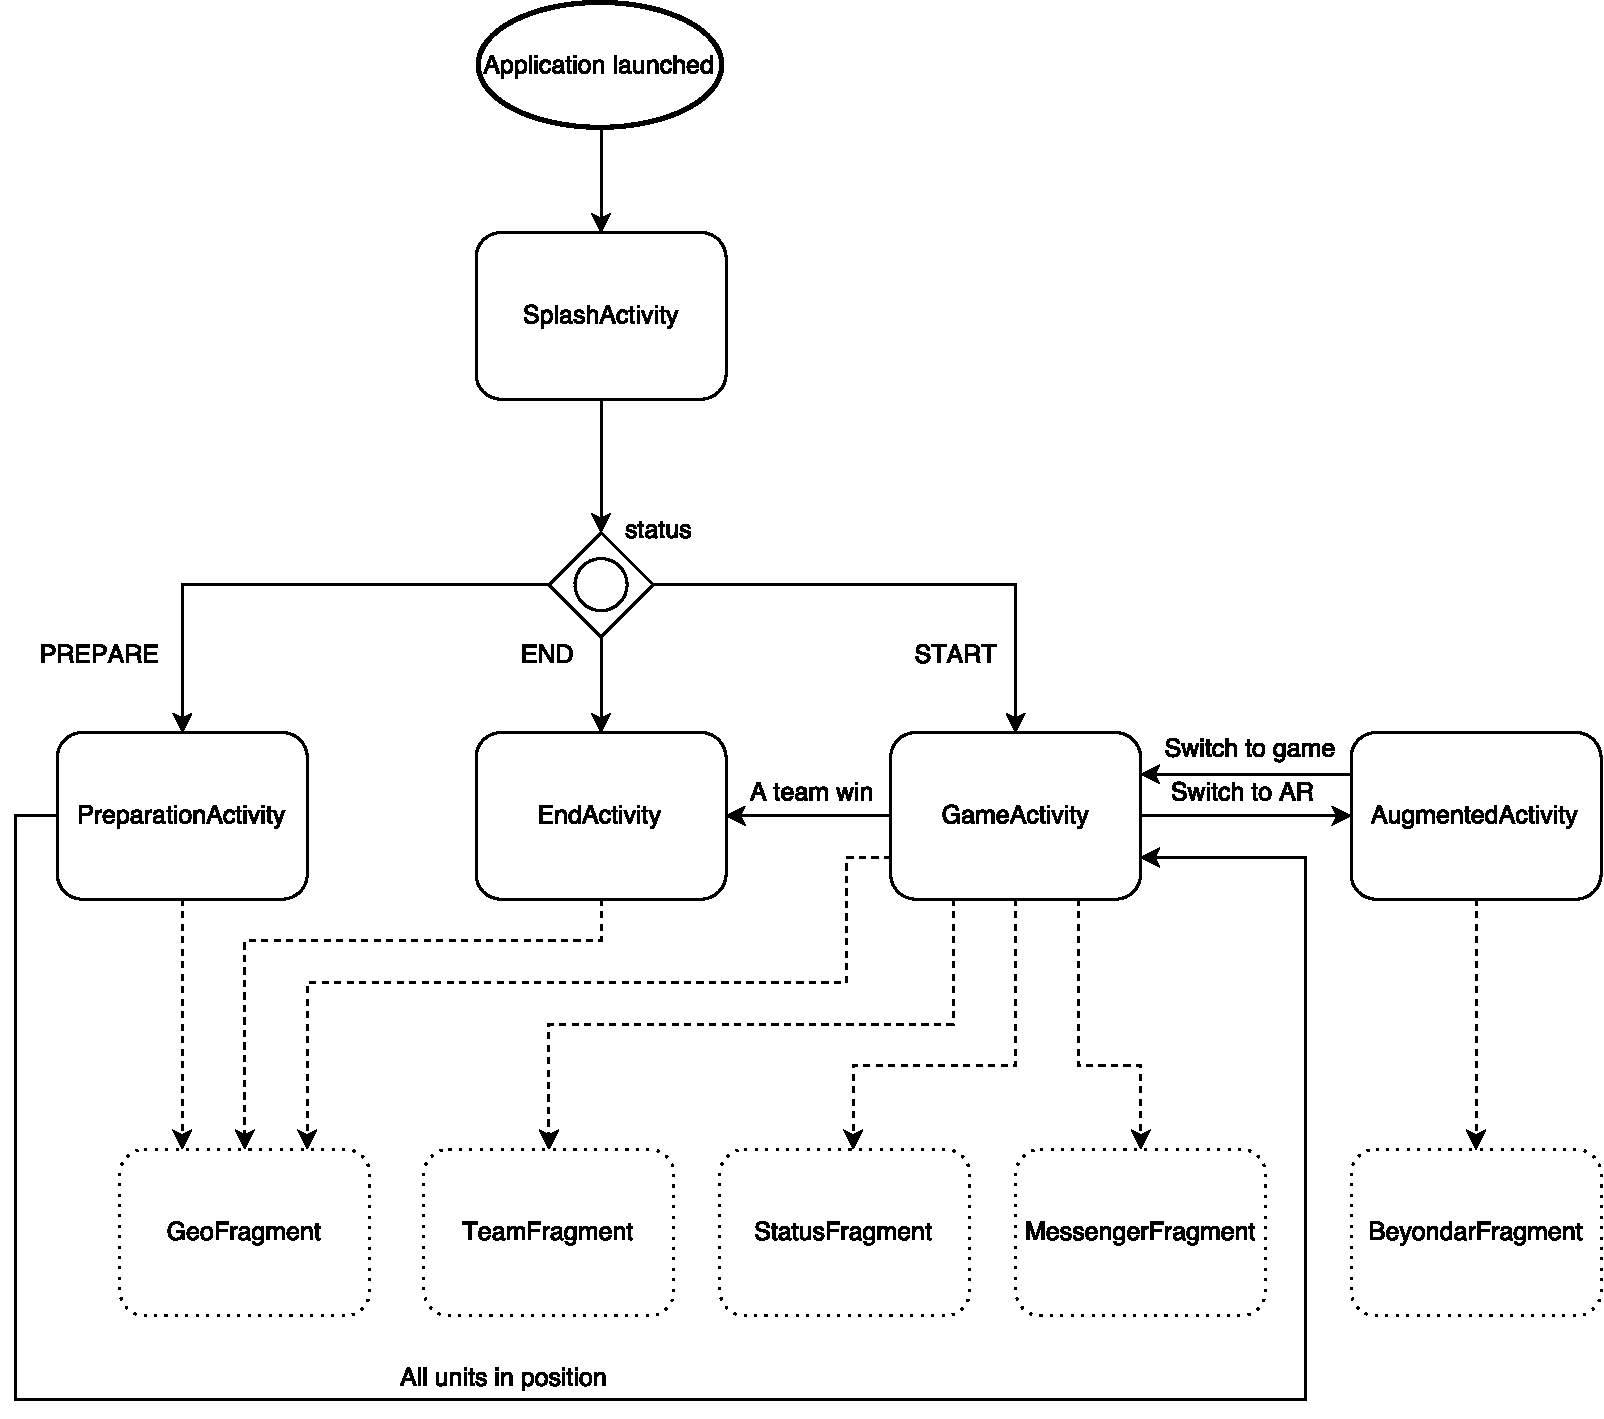
\includegraphics[width=\textwidth]{androidflowchart}
		
		Together with the game mechanics and rules description, a prototype of the game has been prepared for Android systems and works from API 16 onward.
			
		Due to limited time and external job constraints, it has not been possible to finish the prototype in time for the graduation session, which is currently incomplete in some of his modules: messenger system has not been implemented, the augmented reality module which relies on the smartphone camera has not been properly connected to the prototype and with the action system, status fragment which should have shown information about other teams has not be implemented, the end game activity has not been implemented (from a practical point of view, it's more or less a copy of the preparation one).
		
		Following, a description of the features of every activity and fragment which composes the application.
		
		\paragraph{SplashActivity}
		
		It's composed by two alternative layouts: login and loading.
		Its main purpose is to perform the user login and pre-load all useful data for the subsequent activity, which will be started after having understood in which status the game is in that moment.
		Everything it does is described in more details in \autoref{focus:splash}.
		
		\paragraph{PreparationActivity}
		
		It's composed solely by an instance of the \lstinline|GeoFragment| and its main purpose is to guide players to their starting point, forcing them to wait there after they reach it. When everybody is in the right place, it starts \lstinline|GameActivity|.
		
		\paragraph{GameActivity}
			
		It's composed solely by a view pager (a group of tabs) which manages various aspects of the game.
		When a team successfully accomplish its objective, the game status is updated from the server and the application moves to the last activity of the game: \lstinline|EndActivity|.
		
			\subparagraph{GeoFragment}
			
			It's the more important fragment of the activity, because it lets you see the board, where other units are and data about the AR layer of the game.
			At code level, it's a wrapper around a \lstinline|MapFragment| (from Google Maps Android library) who takes care of managing the board and the zones of which it's composed, units position and the related visibility rules, AR objects which spawns around and many others tasks: its workflow is described later in \autoref{focus:map}.
			
			\subparagraph{TeamFragment}
			
			It's composed by four parts, each visible only during certain phases except the forth one:
			\begin{description}
				\item[role management] displays the roles available during the \emph{ROLE} phase and let the unit to select its own;
				\item[action management] displays the actions available, related to the chosen role, during the \emph{ACTION} phase and let the unit to select its own;
				\item[money management] shows how many coins are present in the team reserve and lets unit borrow some of them in the \emph{MONEY} phase;
				\item[teammates status] a list showing the role, action and borrowed money of every unit in the team, it's visible in all phases of the game.
			\end{description}
			
			With this components, the activity manages three out of four phases by which the game is composed.
			
			\subparagraph{StatusFragment}
			
			It's composed by a general status bar, which shows some important data about the game (current turn, how many and which random events are left, etc.), and a list of team summary cards, one for each team playing (number of controlled zones, total money in their reserve, etc.).
			
			\subparagraph{MessengerFragment}
			
			It's similar to every other messenger system (Whatsapp, Allo, Facebook Messenger) and is implemented using the Firebase Cloud Messaging, not needing all the more advanced features (eg. photos and videos).
		
		\paragraph{AugmentedActivity}
		
		It's a \lstinline|FrameLayout| containing a \lstinline|BeyondarFragmentSupport|, a wrapper of a normal fragment enhanced to display the camera captures as background, and an AR overlay which displays things based on the position of various objects and units.
		It's work is to allow interaction amongst units and between them and AR objects, its behaviour is better described in \autoref{focus:augmented}.
		
		\paragraph{EndActivity}
	
		It's the last activity of the game, and it's composed solely by an instance of the GeoFragment as in \lstinline|PreparationActivity|.
		Its main purpose is to gather players to the end position, where the winner will be awarded. When everybody has reached it, the game is finishes and the application force a logout of all players, changing the game status to \emph{INACTIVE}.
	
	\section{Main technological issues}\label{focus:general}
		
		While working on the project, some particular or complex problems required a not trivial solution, which resulted in some interesting pieces of code.
		Hopefully, the explanation about how they were solved here will be helpful for someone who'll need to follow this same path in the future.
		
		\subsection{Board generation}\label{focus:board}
		
			While translating the rules from \textbf{Discworld - Ankh-Morpork} to the mobile game, the definition about how the board should have been, as seen in \autoref{design:board}, took some time.
			
			The initial idea was to obtain a randomly generated, asymmetric board contained in an irregular polygon defined by the event organizers.
			In this way, the playing ground could have been set to fit into different real-world city-related shapes (in Reggio Emilia case, the irregular hexagon made by the beltway was the most obvious shape to use).
			In addition, a randomly generated board would have prevented teams to study strategies based on a fixed map and would have forced them to improvise a new strategy while studying the map in \emph{PREPARE}.
			
			Unluckily, this kind of board generation almost immediately looked too advanced to be realized in the short time available, in its place it has been deployed a more simple regular shape automatically derived from specified centre and radius.
			
			The simplest regular polygon that could be used was of course a circle, and that was the first choice until Google Maps polygons management got in the way. Circular shape was perfect for the board perimeter by himself, but zones perimeter where also needed for others in-game mechanics (checking in which zone each unit is, managing zone crossing, random point generation inside a given zone, etc.) and this was impossible to archive using the build-in circular shape of Maps API.
			The second thought was to replicate the external circular shape with polygons formed by a lot of points, but that would have leaded to possible performance issues, given the number of points needed.
			In the end, as seen in the board image in \autoref{design:board}, a particular shape has been chosen in which the central zone is composed by 8 sides (one vertex every 45 degrees), four more zones are contained between the first zone perimeter and a ring composed by 16 sides (one vertex every 22.5 degrees) and last 4 zones are contained between the first ring and a second ring composed by 24 sides (one every 15 degrees).
			Zones between the second ring and the first one are shifted by 45 degrees because every zone must touch at least other 4.
			
			The fastest way to obtain all zones vertices, possibly also the simplest way apart from hard-coding their GPS positions, is to directly calculate the perimeter of every ring (the two mentioned earlier plus the central zone perimeter), putting all vertices in a multidimensional and ordered array representing zones perimeters.
			This is possible thanks to the fact that zones are all adjacent, which means that many vertices are in common with multiple zones, it's only necessary to put them in the right order.
			
			At code level, this is achieved with three \lstinline|for| loops pretty similar one to the other, which seems to suggest that the procedure could be optimized even further by using polar coordinates, but the code is already complex as it is and for now the result is acceptable.
			The first and last loops calculate vertices clockwise, while the middle loop does it anti-clockwise; this is done because having alternately spinning loops makes much simpler to save vertices of all zones already ordered and get a closed shape for the polygons, as seen in \autoref{board:alternate}.
			
			\begin{figure}[htp]
				\centering
				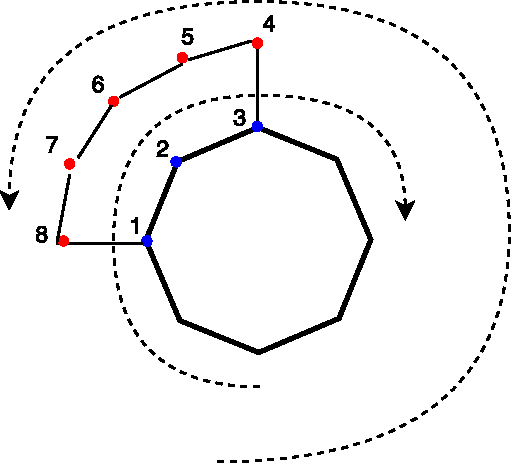
\includegraphics[width=.5\textwidth]{boardrounds}
				\caption{Graphical representation of alternate vertex calculation, showing the perimeter of one of the zones of the first ring}\label{board:alternate}
			\end{figure}
			
			Inside these loops, all points are obtained by starting from the board centre and calculating the new point based on the radius of the given ring and the offset angle which change at every iteration.
			
			\lstinputlisting[caption={Utility method, get new GPS position from given point, distance (ring radius) and angle}, firstline=158, lastline=171]{main/listings/boardfactory.java}
			
			It has to be noted that the board perimeter is not saved anywhere: only zones polygon are stored and printed upon the Google Map, for various reasons.
			First of all, single zones polygons on the map must be able to notice click events for some in-game mechanics (mostly getting zone data, like which teams owns its power-up or how many other units are present in the zone), so they must be saved anyway in order to manage click listeners on them.
			Secondarily, the only feature which requires the board perimeter is the check about someone exiting it, but we can achieve the same result by checking if a position is inside any of the zones which have been saved: if it's not, the unit exited the board.
			
			\begin{figure}[htp]
				\centering
				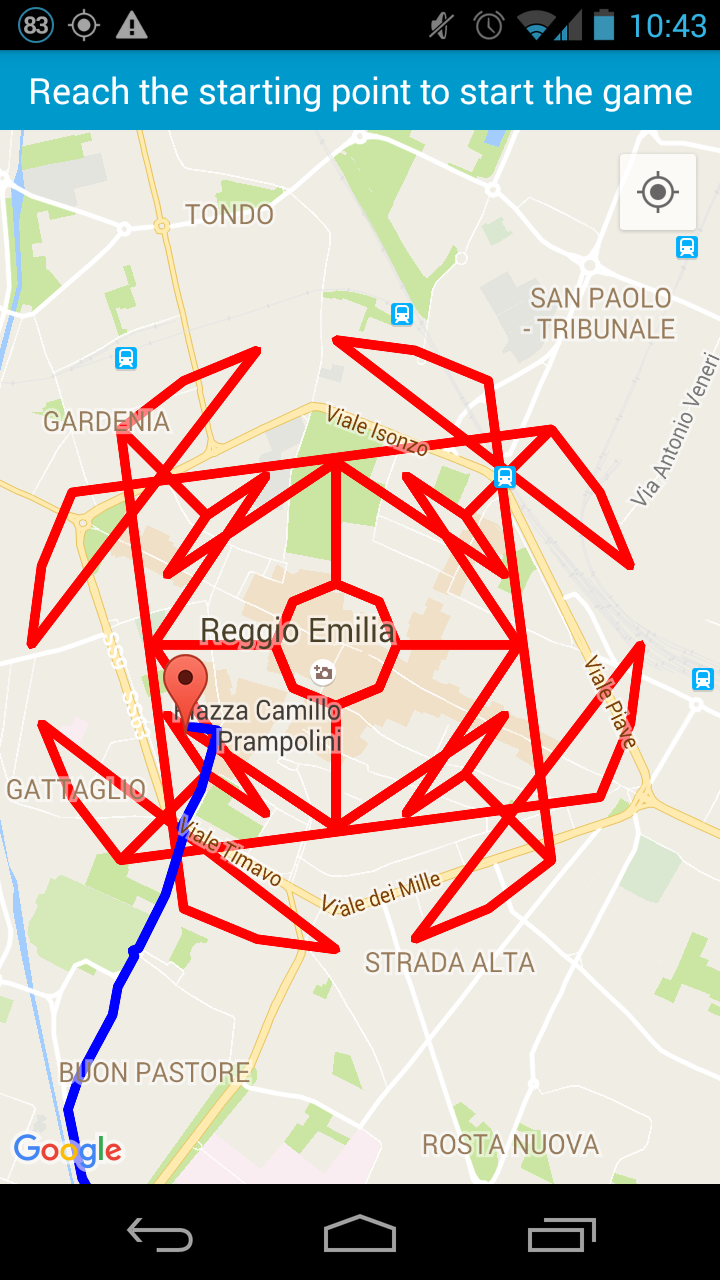
\includegraphics[width=.3\textwidth]{wrongboard1}
				\hfill % Stretches the space between images to align them to borders
				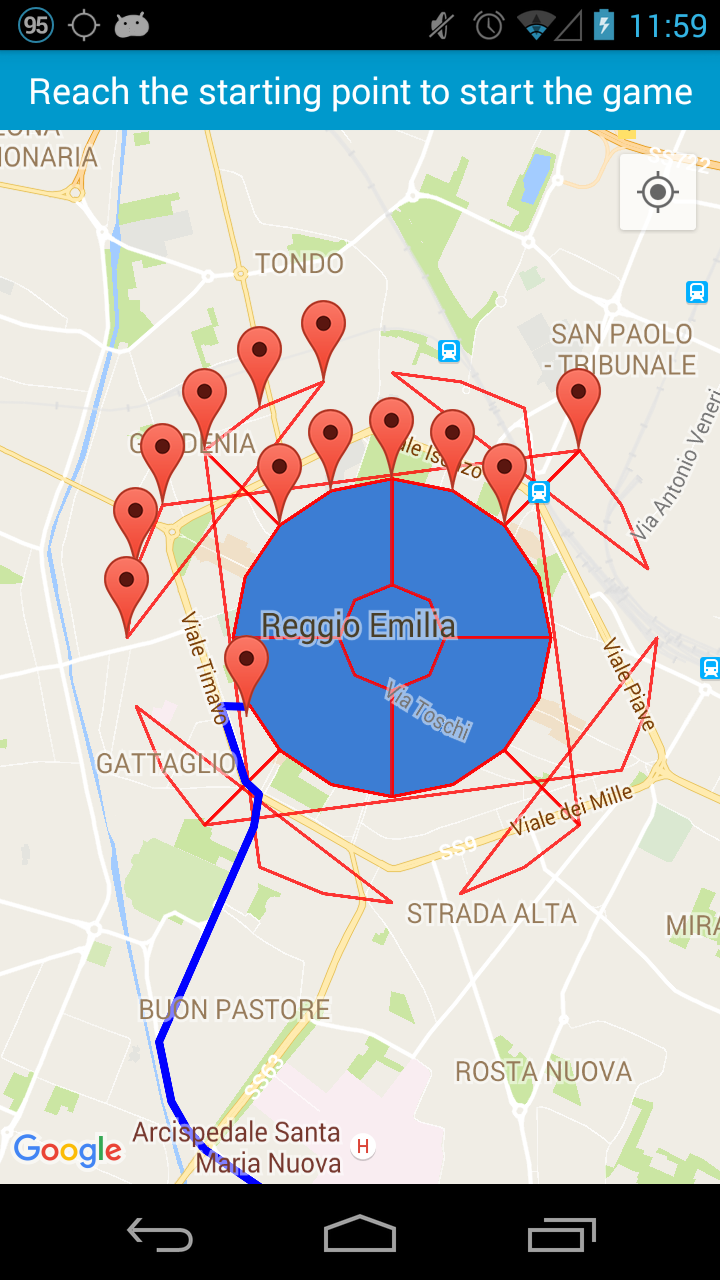
\includegraphics[width=.3\textwidth]{wrongboard2}
				\hfill
				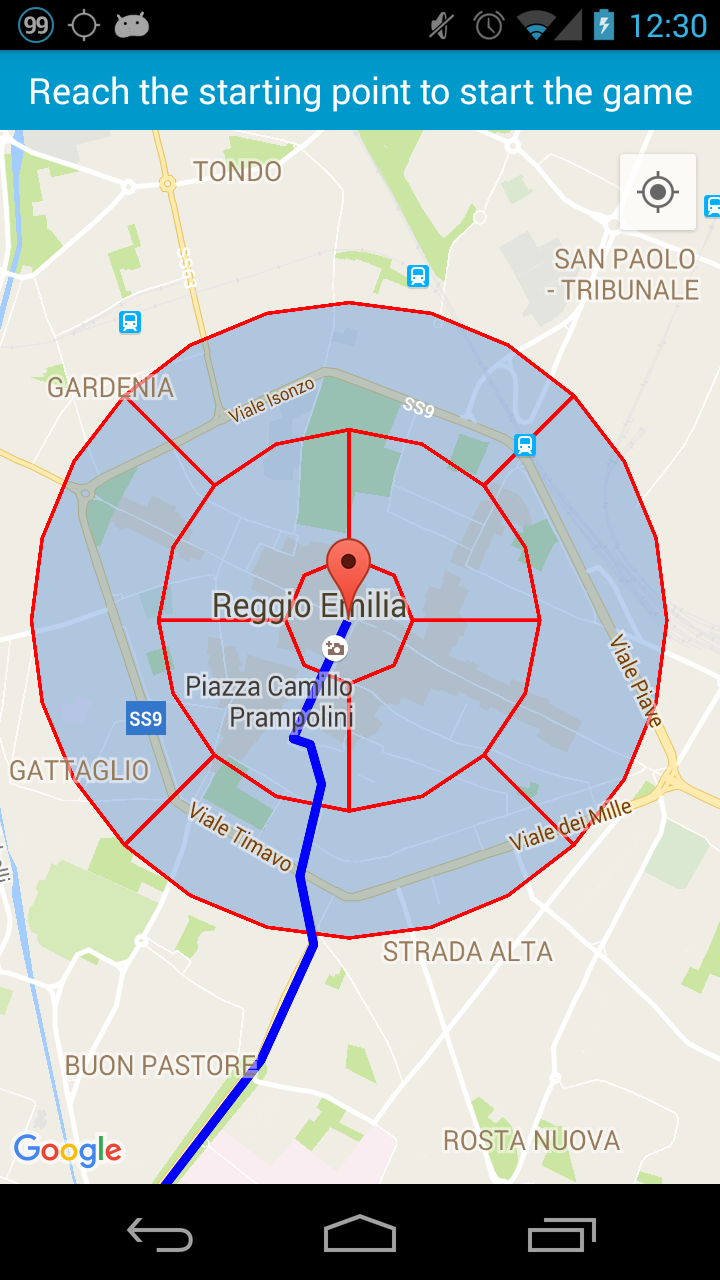
\includegraphics[width=.3\textwidth]{wrongboard3}
				
				\caption{Three board drawings trials while developing \lstinline|BoardFactory|}\label{board:mess}
			\end{figure}
			
			After some trial and error (\autoref{board:mess}), the right shape has been obtained, but the radius used to calculate the rings was obviously wrong.
			Considering that zones must have the same area, an R script has been used to find out which radius every ring should have had. Obviously the R script assumed the rings as circles, not as the weird shapes they actually are.
			
			After loops finish their run, the multidimensional array is used to fill in the perimeter \lstinline|ArrayList| of every zone on the board.
			
			The last part of the board fabrication is to make all zones aware of their neighbours. Unluckily, here hard-coding seems the only viable way, and for now the map is simple enough to allow for this.
			
		\subsection{Timer mechanism}\label{focus:timer}
		
			Synchronizing phases between server and clients is pretty easy with Firebase: taken that the server manages phase timers by his own without crashing and updates accordingly the phase field on game branch, devices just need to set a listener on it in order to know in which phase the game is.
			The task become less trivial when you add the fact that all devices must have a synchronized countdown of the current phase.
			
			The first idea was to store, together with the current phase, also the timer duration.
			In this way, every device connected could just set an internal timer, nearly synchronized with the one on the server and the problem was solved.
			
			But let's go further: what if the devices must be able to connect/disconnect at will and still have the synchronized countdown feature?
			The must obvious idea would have been to add another field, perhaps the moment in which the timer started, together with his duration.
			
			To spare a field (which, in Firebase, usually means sparing an asynchronous callback and a lot of trouble), the solution was to store, instead of starting time and duration, directly the expiration moment of the timer.
			For this to work, the time on every device and on the server must be the same. This is usually automatically managed by the operating system which uses internet to synchronize himself to the right time and can be took as assured on the server machine, but on players smartphones internal time could be modified by the users, which open the gates to possible glitches and cheats.
			
			Luckily Firebase comes to assist us on this as well: listening to the particular path \lstinline|.info|, a number of miscellaneous and useful piece of data can be accessed, one of them being the time offset between the local device and the Firebase server local time.
			
			Listening to \lstinline|.info/serverTimeOffset| value changes allow us to detect the current offset from the server, store it and add it to the countdown timer that displays the remaining time at every timer field change or device connection.
			
			To prevent every possible exploit, every time the timer field is changed on Firebase by the server, the local timer on every device is cancelled (if it was not expired yet), his onFinish callback executed and the new timer is set up.
		
		\subsection{Match logging}\label{focus:log}
		
			In order to better study the game mechanics effectiveness, it can be useful a replay feature, which can be used also to detect cheaters or problems.
			
			For this, a logging system has been prepared, which keeps track of all units' actions, as well as their movements, and various in-game events.
			
			The \lstinline|GameLogger| class is a singleton that statically provides a logger which writes to a file in the "/log" path, appending the creation timestamp to the log file name to log multiple game sessions.
			
			All server model classes implements the \lstinline|FirebaseSync| interface, which ask to override the \lstinline|sync()| method.
			In this method, called at the end of the constructor, all listeners to useful data from Firebase must be set.
			In this way, all instances will auto-update themselves, listening for changes on Firebase, and while doing so they'll also log all the meaningful actions and events which will be taking place during the match.
			
			When the game finishes, the structured log file could be set as input of an ad-hoc decoder, reproducing the events like a video.
			
			This ad-hoc decoder has not been developed yet, but shouldn't be hard to implement. 
		
		\subsection{Random picker}\label{focus:picker}
		
			\lstinputlisting[caption=Random picker class]
							{main/listings/randompicker.java}
			
			A small but useful function which is missing from Java \lstinline|List| interface implementations is the possibility to extract a random object from a given list.
			This may seem a bit useless, but nearly all games may need some kind of random extraction and also in other contexts (eg. testing purposes) a small feature like this can come handy.
			
			In this project, randomly assigned values are used in many parts, eg. objectives distribution to teams, and a lot of parts not yet completed will heavily relies on random generation and extraction.
			
			For this reasons, a small utility class has been written to extract random values from a given list. It exposes two methods:
			\begin{description}
				\item[pick] takes the random seed of this thread, then randomly picks an integer value between 0 and the list size -1 and returns the list element associated to that value. 
				\item[extract] same as \lstinline|pick| method, but removes the extracted object from the list before returning it.
			\end{description}
		
			The picker uses \lstinline|ThreadLocalRandom| class instead of the more known \lstinline|Random| because, relying on asynchronous callbacks and on multi-threading, the synchronized access overhead to the process-global class may decrease performance a little.
			Plus, it's the recommended class to use, as written in Java 8 docs.
						
		\subsection{Random point generation}\label{focus:point}
		
			\lstinputlisting[caption=Random point generator class]
							{main/listings/randompoint.java}
			
			To implement most of the AR interactions, a way to generate random points, usually inside a given zone perimeter, it's needed.
			
			Generating coins inside every zone for the collectors, drawing a path composed by random points to calm a zone or make it chaotic and other actions, rely on this function.
			
			On Android, it's easy to get the previously saved Polygon of a zone and generate a point within its bounds, checking later if the point is actually inside its shape\footnote{Let's remember that a Polygon shape and its bounds are not the same thing: the shape can be irregular, while it's bounds are the smallest rectangle around the shape which contains all its points} with Google Maps PolyUtils support library, but on the server we do not have such a powerful tool.
			
			The \lstinline|RandomPoint| class has been written to address this deficiency.
			
			Given as input a generic perimeter (this can also be the board itself or an area around a given player), the method will generate a \lstinline|Path2D| region from it, giving access to the \lstinline|Path2D.contains(x,y)| method.
			
			Then it will get the region bounds and keep selecting a random point inside that rectangle until the point we got is actually contained inside the given region.
			
			Once an acceptable point is found, it is returned wrapped in a \lstinline|GeoLocation| object.
		
		\subsection{Zone control manager}\label{focus:control}
		
			The \lstinline|ControlObjective| needs a special mechanics to understand which team currently controls a given zone.
			A zone is controlled by a team if the sum of its buildings and units there is greater than the one of every other team.
			If two or more teams have equal sum, nobody controls the zone.
			In the Firebase data model, the controller team is specified in the \lstinline|controller| field, which is updated by the server.
			In fact, every time a unit changes zone or a building is constructed/demolished the server replicates that information on the selected zone instance using the \lstinline|addUnit|, \lstinline|removeUnit|, \lstinline|addBuilding| and \lstinline|removeBuilding| methods.
			Every one of those, after updating their own \lstinline|ArrayList| of units/buildings, calls \lstinline|updateController|.
			This method, which ask for a team reference and an integer as parameters, updates the control \lstinline|HashMap| which keeps track of the sum of buildings and units of every team, then search the entry where that value is the maximum.
			Every time a new maximum is found, its team reference (which is the key of the \lstinline|HashMap| entry) is stored as the controller team, but if a second entry with the same value is found, the controller team reference is set to null.
			After cycling all the entries, the controller variable is set to the right team reference (or null if no one controls the zone) and it's accessible with \lstinline|getController| method.
		
		\subsection{Presence system}\label{focus:presence}

			It's important, both for teammates and enemies to be able to see if a given player in their zone is currently active (eg. is using the application, it's GPS position is accurate) or not.
			
			Using Firebase, setting up a presence system is trivial, thanks to official guides\cite{firebase:presence} and ad-hoc tools provided by the library.
			
			The \lstinline|OnDisconnect| object can be chained with the \lstinline|Query| one to store a particular operation on the server, which will be executed when the connection with the client interrupts.
			
			Considering that the presence system is required in 4 different activities it has been put in a singleton class, \lstinline|PresenceManager|, which exposes two static methods: \lstinline|PresenceManager.setup(userId)| and \lstinline|PresenceManager.cancel()|.
		 
			\paragraph{setup}
			Initializes the presence manager using the given user id.
			If the singleton has already been initialized, the user id is checked against the previously saved one: if it's the same, no operation is done  and the presence manager is shared between different activities saving some overhead, otherwise the \lstinline|cancel| method is called and a normal set-up takes place.
			If instead it's the first initialization, the user id and some disconnection listener references are stored internally, then a value listener on the particular location \lstinline|.info/connected| is added: like many informations on the special \lstinline|.info| branch, this value is updated directly by Firebase, in this case every time the client's connection state changes.
			As soon as the \lstinline|.info/connected| callback is fired with value \lstinline|true|, a new branch with the user id as key is pushed into the \lstinline|presence| branch (see \autoref{model:presence}) and two operations are stored on the server to be executed upon disconnect event: the first one removes the value from \lstinline|presence| branch, while the second updates \lstinline|lastOnline| field inside the user personal branch.
			In this way, it's easy to check which users are currently connected reading  \lstinline|presence| branch children, and it's easy as well checking the last moment in which a particular user disconnected.
			
			\paragraph{cancel}
			If the singleton has actually been initialized, resets the presence manager removing all values and disconnect listeners.
		
		\subsection{Splash screen and data pre-loading}\label{focus:splash}
		
			To avoid long loading times once inside the application, most of the common data to all activities are retrieved in the splash activity, which also manages players login.
			These data are stored into the shared preferences or sent as extras attached to intents.
			
			The splash screen is composed by two alternatively shown layouts: login and loading.
			Login layout shows the application icon, email field, password field and login button.
			Loading layout instead it's not interactive and shows a loading animation and a text component which inform the user about which operations are being performed.
			
			Numerous steps must be executed before the application can start flawlessly:
			\begin{itemize}
				\item perform login or auto-login;
				\item retrieve unit and team id;
				\item enable GPS;
				\item retrieve current location;
				\item check game current status.
			\end{itemize}
			
			\paragraph{Login}
			By default, the loading layout is the visible one, considering that thanks to an auto-login feature the login layout is visible only for the first access or if an error occurs.
			The email and password are stored in shared preferences after the first login and automatically inserted into the appropriate fields in the subsequent accesses: if both email and password are actually present, the auto-login feature is turned on.
			
			When auto-login is not enabled, login layout is shown in place of the loading one and the user is prompted to insert email and password, which will be then used to initialize a Firebase Auth session.
			
			Firebase Auth natively provides a token-based auto-login feature, but its implementation is buggy so, after the Firebase Auth system initialization, his attempt to perform it is blocked and, if needed, the home-made one is activated.
			
			The auto-login home-made implementation uses previously saved credentials (losing some security with respect to the token-based system), to simply perform a normal login procedure, but automatized by the code.
			
			After the login completes successfully, the \lstinline|lastOnline| field of the current unit is updated.
			
			\paragraph{Unit and Team IDs}
			
			Unit id and team id are crucial for all activities: they're used in \lstinline|GeoFragment| (used in \lstinline|PreparationActivity|, \lstinline|GameActivity| and \lstinline|EndActivity|), \lstinline|TeamFragment|, \lstinline|AugmentedActivity|, etc. Those are almost \emph{all} the important parts of the application.
			If every component had to retrieve them by his own (as it were at an earlier stage of the project), the code would have been a mess, with duplicate code in every class performing a call to the Firebase Auth system to get the user id and then to Firebase Database to get the team id using the previously retrieved user id.
			For this reason, those IDs are directly retrieved right after the login and stored in the shared preferences in order to be accessible in every activity of the application.
			
			When performing the login, user id comes for free: during unit branch creation, its id is set as the same from Firebase Auth system, so it can be retrieved using \lstinline|FirebaseAuth.getCurrentUser().getUid()|.
			Team id is retrieved right after, using a specific Firebase Database request upon the unit branch.
			
			\paragraph{GPS}
			
			Being a location-based AR, the GPS service must always be enabled while using the application, so the first thing to do is to switch it on.
			To do so, \lstinline|GoogleApiClient| must be initialized first and the system location service can then be retrieved.
			If its GPS provider is already enabled (which means, if the GPS feature is turned on), this step can be skipped, otherwise the provider must be activated: a new dummy \lstinline|LocationRequest| is created and launched, thanks to the previously initialized \lstinline|GoogleApiClient|, to check if it can be activated.
			If the request says the GPS can be enabled,  \lstinline|startResolutionForResult| method provided by the GMS API is used to ask the user the permission to enable it on his behalf, otherwise there is a problem with the GPS provider which cannot be resolved: the error is notified to the user and the login layout displayed.
			If the user declines the request of turning on the GPS, an error is displayed and he's kindly asked again to do so, until he accepts.
			
			\paragraph{Current location}
			
			Having obtained GPS permission, \lstinline|FusedLocationApi| is used to get the last known location of the device with  \lstinline|getLastLocation| method.
			This powerful tool gets all location service providers available in that moment (cellular network, Wi-Fi, GPS, smartphone sensors) and mix their data in order to get the most accurate position obtainable, exposing a simple API which can let the developer define which retrieve mode must be used (low battery consumption, high accuracy, etc.) while reducing at his best battery drain.
			The last known location is kept by Android system, which saves the value of the last position retrieved by any application or service using Google Play Services on that device.
			Having retrieved a more or less accurate unit's current position, it is stored and the last step of the initialization procedure is performed.
			If there is no last known location (\lstinline|getLastLocation| returns a null pointer), a \lstinline|LocationRequest| is set up and launched to retrieve it.
			
			\paragraph{Game status}
			
			Considering that the game can have any status when the user access the application, the last step is to query Firebase Database to check the current status and start the next activity accordingly.
			If the game has \emph{INACTIVE} or \emph{INITIALIZE} status, the user is noticed that the game cannot be accessed yet.
			If it has \emph{PREPARE} status, \lstinline|PreparationActivity| is started, which helps the players to display correctly on the game board.
			If it has \emph{START} status, \lstinline|GameActivity| is started, which manages the entire game.
			If it has \emph{END} status, \lstinline|EndActivity| is started, which informs all players of who won the game and gathers them to a common place where the winning team will be awarded and the event will continue.
		
		\subsection{Navigation drawer template}\label{focus:drawer}
		
			Even if the final version of the application does not include a navigation drawer, the absence of a simple yet flexible implementation of it, which could be applied smoothly to multiple activities, is puzzling.
			Moreover, the project needed some kind of template to avoid to rewrite the common frame of all activities (coordinator layout and his behaviour, action bar, information bar).
			Given this, an implementation of it had been realized.
			
			All findable guides about this topic are based upon defining every single activity as implementing the navigation drawer interface.
			A more advanced idea is to define an abstract class which extends the activity class and implements the navigation drawer interface, making all activities extend it.
			In this scenario, the activity must call an initializer function in his \lstinline|onCreate| method, which could lead to oversights and errors difficult to track down. Moreover, the \lstinline|setContentView| is still delegated to the activity, meaning that its XML layout code is still product of the copy/paste of all navigation drawer views between an activity's layout file and the other.
			
			The developed solution is still sort-of based on this idea, but is more general: the \lstinline|NavActivity| abstract class load an XML layout with the navigation drawer feature, which in turn include a second XML layout with all other frame components.
			This division let the developer see in Android Studio preview how the frame graphics will be both with the open navigation drawer and the closed one.
			\lstinline|NavActivity| takes care of the common operations to every activity, mostly initialization and management of action bar, information bar and navigation drawer.
			The XML template layout is a \lstinline|CoordinatorLayout| whose children are an \lstinline|AppBarLayout|, a \lstinline|FrameLayout| and a toolbar which acts as information bar.
			The \lstinline|FrameLayout| is a place-holder, it is set as content view and sub-sequentially the specific activity layout is inflated inside it.
			
			To know which layout we have to inflate into the template, an abstract method called \lstinline|getContentLayoutId| is defined.
			All activities extending \lstinline|NavActivity| are forced to implement this method which must return the id of the layout to be inflated, this avoid possible oversights.
			
			This system also reduce code redundancy and copy/paste actions to zero, removing one of the major errors generator while coding.
		
		\subsection{AR on map}\label{focus:map}
		
			One of the most complex yet fundamental challenge which had been faced, was the definition and creation of the \lstinline|GeoFragment|: a class wrapping the \lstinline|MapFragment| from Google Maps API and over which half of the application AR layer had been built.
			
			The main problems bound to this component were the continuous retrieving of the user position, other players tracking and displaying, and the implementation of the visibility rules amongst users or between users and AR objects.
			
			Additionally, as described in \autoref{app:workflow}, this component is used in three different activities: \lstinline|PreparationActivity|, \lstinline|GameActivity| and \lstinline|EndActivity|.
			The problems are the same for all activities, but must be managed differently based on which activity is instantiating the fragment.
			
			Other tasks performed by this component, either trivial or already discussed in other parts of this document, are: map customization, zones download and board drawing, team color download and markers pre-loading.
			
			\subsubsection{Location sniffer}
			
			\lstinline|MapFragment| by his own already comes with an easy to activate and use \emph{My Location} layer, which saves us some trouble while adding some others.
			In fact, the default \lstinline|LocationSource| used for that layer is an internal one from which is not possible to get the location updates from an external piece of code: once it's been set up, the location updates are directly sent to the \emph{My Location} layer without an access via some kind of API.
			This meant that either the entire layer should have been recreated or two location service requests had to be activated. They were both unpleasant options, a more graceful third one had been searched, and found, which consist in a new utility component which implements the \lstinline|LocationSource| and \lstinline|LocationListener| interfaces and replicate the Google internal \lstinline|LocationSource| implementation as best as possible; this component, called \lstinline|LocationSnifferSource|, takes as parameters the activity to which is bound and an object implementing the \lstinline|LocationSniffer| interface (usually the activity itself), and sends every location retrieved to the sniffer class right after sending it to the rightful object that activated the location source (in this case, the Google \emph{My Location} layer).
			
			In this way we are piggybacking on the location which would  have been retrieved anyway by the \emph{My Location} layer avoiding to ask for a location twice every time or to re-implement that layer.
			
			This component is then set as the \lstinline|LocationSource| which must be used by the Google Map component; this also prevent leaks, because the location source will be activated and deactivated automatically by the Google Map upon \lstinline|onStart|/\lstinline|onStop| methods of the \lstinline|MapFragment| life-cycle.
			
			\subsubsection{Other players tracking and displaying}
			
			Considering that every unit in game \emph{could} be visible over the board at any time and that the visibility rules change as the game phase or status do so, players are tracked storing all theirs data but activating a listener on their position only when they must really be shown on the board.
			
				\paragraph{Unit model}
					
				In order to keep the data of the units related to their representation on the map, a private class has been created: \lstinline|UnitData|.
				This class holds unit general information (id, team, role) together with some data related to the location of the unit (GPS position and current zone), a reference to his marker and a location listener one.
				
				Role and current zone are automatically updated when they change on the database, this automatic sync is vital to the visibility system.
				
				The location field represent the last known GPS position of the unit, while the location listener reference is added or removed depending on when unit must be visible or not (we do not need to keep track of the movements of units we cannot see).
				
				The marker reference is used when the unit last known location is updated, causing the marker itself to move on the board or, when a unit disconnect, causing it to become partially transparent.
			
				\paragraph{Unit initialization}
				
				During the first setup of the fragment, an \lstinline|HashMap<String,UnitData>| is filled with an entry per unit in game.
				This entry, referenced by the unit id, is filled with the id, the team and the current role of the unit.
				The unit is initially assumed to be out of the board, so we set the zone equal to 0: a listener is then added to keep the zone value synchronized with the database.
				We set the current position to a dummy \lstinline|LatLng| in (0,0). This is needed because we are not sure that the unit currently have a position set on the database, but we \emph{must} provide one where to place the marker on the board.
				The marker icon is a circular dot with the color of the team of the unit, it's title is the unit username and by default is set as not visible.
				
				A listener is added to keep the unit role in sync with the database, while another one keeps track of the presence of the unit (changing the transparency of the marker accordingly).
				
				Units which are in the same team as the current user are automatically set as always visible, and their location listener is activated.
				
			
			\subsubsection{Visibility rules} \label{focus:map:visibility}
		
			Obtaining a clean code while managing the visibility rules had been an hard task, and several structure rethinks were needed before finding an acceptable solution.
			This would have been trivial if all units could just see everybody else, but the idea was to limit their sight in order to force collaboration and communication amongst teammates and to push them into trying to foresee other team movements from incomplete data.
			This is why the visibility rules change accordingly to the game phase: while in \emph{TURN} phase the sight is limited and they must make assumption on what other teams are doing, in any other phase all units are visible, in this way the players can check if their assumption were right and can access the whole picture for some time in order to continue this prediction mind game.
			
			\begin{table}
				\caption{Visibility rules}
				\label{focus:map:visibility:rules}
				\centering
				\begin{tabular}{lcccc}
					\toprule
					\multirow{2}*{Game status} & \multicolumn{4}{c}{Current user role} \\
					\cmidrule(lr){2-5}
					& \emph{COP} & \emph{ASSASSIN} & \emph{BUILDER} & \emph{COLLECTOR} \\
					\midrule
					\emph{PREPARE} or \emph{END} & \multicolumn{4}{c}{Everyone, in all zones} \\
					\emph{START} not in \emph{TURN} phase & \multicolumn{4}{c}{Everyone, in all zones} \\
					\emph{START} in \emph{TURN} phase & \emph{ASSASSIN} & \emph{BUILDER} & Everyone & No one \\
					\bottomrule
				\end{tabular}
			\end{table}
			
			The visibility rules are summarized in \autoref{focus:map:visibility:rules}: while the most are just a matter of enabling/disabling location listener of all the units and show/hide the respective markers, the most interesting to analyse are the ones of \emph{TURN} phase, which are applied in two step. 
				
				\paragraph{Zone limitation}
				
				The user sees only the units in his own zone (except from his teammates which are always visible). Initially, this has been done setting a listener on the zone field of every unit and checking if they were in the same one as the current user, but it proved to be an infeasible solution given the growing complexity of managing consistently a lot of listeners related to a vital aspect of the application.
				The current solution is based on the fact that every player, upon his device GPS position change, updates his current location and checks by his own in which zone he's in, updating that piece of information as well.
				While doing so, the user now updates also the list of users present in a zone, both for the zone he's entering, adding himself in, and for the one he's exiting, removing himself from it.
				Listening to that users list of any of the zones automatically inform the current user of which marker he can show, provided that the listener changes the target zone accordingly to his movements.
				To avoid possible "flickering" when an user is on the border of a zone, a delta value is added to the check (10 meters) and must be surpassed to actually change the active zone.
				
				\paragraph{Role limitation}
				
				The user sees only some kind of other units, as shown in \autoref{focus:map:visibility:rules}.
				This is accomplished with a rule \lstinline|HashMap<Role,Role>| which, given as key the current user role, select which role must have the other units to be visible.
				This is a limitation but also an useful information: if you are a cop, you know that all the enemy units you are seeing in the zone are assassins, for example, and act accordingly to protect your teammates.
				
		\subsection{AR on camera}\label{focus:augmented}
			
		While the map is all a matter of \emph{seeing} AR objects and other units, the actual interaction with the augmented world take place in \lstinline|AugmentedActivity|.
		This activity is composed solely by a \lstinline|BeyondarSupportFragment|, which by his own is a \lstinline|GLSurfaceView| with transparent background, where AR objects are rendered, placed in front of a common \lstinline|SurfaceView|, where the frames caught by the camera are redirected. In this way we can see the AR objects placed in the real world, based on their GPS position and other device sensors.
		
		This activity is accessible via the \lstinline|GameActivity|, and a button is displayed to take the user back there when he's done using the AR module.
		It's important to note that this activity is accessible only during the \emph{TURN} phase while the game is in \emph{START} status: if the user is in this activity when the timer expires, it will be automatically redirected on the \lstinline|GameActivity|.
		
		While the concept of zone is less relevant in this mode, because the visibility rules does not involve them, a simplified version of the system used in \lstinline|GeoFragment| is re-used here as well, in order to keep data on Firebase up to date.
		
		Also the phase timer, more useful than ever in this mode, is retained from \lstinline|GameActivity| but displayed in a more discreet way.
		
		The work flow of this activity is pretty straightforward: when started, it requires the objects within a certain radius around the given initial location and use them to initialize a \lstinline|World| instance, an abstraction provided by the Beyondar framework.
		Then it's registered a location request to keep the position of the player updated inside the \lstinline|World| representation, while other players and AR objects will be added/removed dynamically from it when they exit the given radius. In case the user tries to disable the GPS sensor, an error message is displayed, he's logged out and it will be asked to re-enable it.
		
		Two main problems have been faced for this component: other players tracking and displaying, and interactions with AR objects and units.
		
		\textbf{Due to time constraints, the second one has not been implemented, just theorized.} 
			
			\subsubsection{Tracking and displaying}
			
			With respect to the map AR part, other players tracking is a lot easier, thanks to an add-on available for Firebase: GeoFire.
			This library allow us to perform geo-queries: query on the database which retrieves all pre-registered objects/players within a certain radius.
			The visibility rule for this component has been thought to be pretty straightforward, given that when using it players will be in the most dynamic moments of the turn phase and people will be probably running around: every player closer than 25 meters from the current user is displayed, with a label on his head which identifies his team and role, and every AR object closer than 80 meters is displayed as well.
			These rules are enforced by two geo-queries, considering the two different rays, which monitor all the entering and exiting players/AR objects and which criteria (the centre of the geo-query) is updated every time a new GPS position is retrieved by the device.
			
			Every unit trying to interact in any way with the AR world will be visible, because in order to access and use the \lstinline|AugmentedActivity| the GPS must be active and the location updates with it.
			The fact that \emph{all} interactions are possible only via this activity limits scenarios in which, for example, assassins reach their prey with the application or GPS turned off to catch it by surprise.
			
			\subsubsection{Interactions}\label{focus:augmented:actions}
			
			Interactions via the augmented reality world can assume various forms, usually some kind of mini-game, and depends from the role and action chosen by the current user.
			
				\paragraph{Follow the path}
				It's the one used for the \emph{CALM} action of the \emph{COP} and the \emph{PANIC} action of the \emph{BUILDER}, which both alter the current zone chaotic status.
				It basically consist in following a path composed by multiple POIs inside the current zone. The points can be actual POIs taken from Google repositories or simply on-the-fly randomly generated points inside the zone by the application.
				An arrow will always points towards the next POI which must be reached, the distance to reach it will be displayed as well, and a graphical effect (depending on the setting of the game) is generated every time one is reached.
				
				\paragraph{Collect}
				It's the one used for the \emph{COLLECT} action of the \emph{COLLECTOR}, which can gain randomly generated coins for his team.
				This interaction resemble the previous one, except that the coins are AR objects shared between all players (once one is collected, it disappears from the display of all others collectors) and must be mined. The mining process can be a tap-hold or multiple taps, the important thing is that the collector must stay over the same coin at least 10 seconds: this creates a weak spot where assassins can recognize them and eventually take them down. The number of collectors already present in a zone is displayed, in case the current player prefers to move to a zone with less collectors, hoping to have less competition while gathering the coins.
				Another difference from the \textbf{follow the path} interaction is that there will be multiple arrows pointing to the three coins closer to the current player, instead of just one.
				
				\paragraph{Stay near here}
				It's the one used for the \emph{PROTECT} action of the \emph{COP} and the \emph{ASSASSINATE} action of the \emph{ASSASSIN}, both related to the assassination mechanism.
				The basis are the same for both actions: when within a certain range from another unit it's possible to mark it as the target of your action, then you have to get near that unit into a smaller range, if you manage to stay within this second range for a given amount of time, your action succeed, otherwise you fail and must repeat the procedure after a cool-down time.
				What differs between the two actions are the meanings and values of the various phases.
				
				
				For the cop, the first range is 10 meters, the second one is 4 meters, the time in which he can stay within 4 meters by his target is 15 seconds and for all that time the cop himself and the protected unit cannot be targeted by assassins (if the unit was already the target of an assassin, the assassination fails). The cool-down of this action is 10 seconds, after which you can re-use it (both in case of failure or success).
				This action is indeed pretty boring if compared to the others, but hopefully it will be mitigated by the fact that who takes it will be always together with at least one of his teammates.
				
				
				For the assassin, the first range is 5 meters, the second one is 3 meters, the time in which he must stay within 3 meters by his target is 4 seconds. If he manages to kill his target, he cannot perform other kills for that turn. If he fails, the cool-down time is 5 seconds, after which he can retry the assassination. He can repeat this until he succeeds or the \emph{TURN} phase timer expires.
				When the assassin select a target, his phone will emit a sound to alert him and, if he's using the application in that moment, the screen will reflect the danger situation.
				
				
				\paragraph{Perform gestures}
				It's the one used for the \emph{BUILD} action of the \emph{BUILDER} and the \emph{DEMOLISH} action of the \emph{ASSASSIN}, both related to the buildings mechanism.
				This kind of interaction must keep who perform it occupied for 1 minute and half or more, giving the importance that this actions have on the game in a lot of his parts (power-ups management, the money usage, the control of a zone, etc.) and consist in a random flow of different gestures which must be executed by the player. If the gesture is executed correctly and with the right timing, it scores a point (or more points in case of combos), if it does mistakes, it loses a point. While this points pool increase, the building object is shown to grow/spoil, depending on the action, on the AR layer, and when it reaches a certain value (150 for example), the building is completed/destroyed and is added/removed from the database and map.
				Gestures can vary from simple touch and swipes to more advanced and particular once, like touch-less gestures and blow recognition offered by some SDKs\footnote{Snapback (http://www.snapback.io/), even if not yet publicly available, can be an interesting partner to add not standard gestures.}.
				Buildings can be constructed only within a radius of 30 meters from the zone centre.
	
	\chapter{Results}

	TODO
	
	\chapter{Conclusion}

	Looking back at the introduction, it is possible to say that most of our objectives had been reached and that the principles defined at the beginning had been respected.
	
	The application is active only during the event and can be placed on the Play Store, considering that users cannot login anyway if they do not own the credentials, which are given only to teams' members who subscribe on-line.
	
	Instead of relying on micro transactions from the users, avoiding the pay-per-win typical behaviour, it is offered to organizations (associations, companies, etc.) willingly to prepare and publicize an event in which the game is the main attraction, but not the only one; the most common use case is to prepare a bundle with dinner, game and possibly overnight stay, offered to organized groups of participants up to 30 people for a single event.
	This kind of events is particularly suitable to bring the attention of the people on the restaurant/pub where the dinner takes place or where the players will spend their night, considering that the game is spatially located in the urban area among common citizens.
	
	Just by reading the rules, it is obvious that the game heavy relies on team play, which was one of the aims: pursuing alone the team's objective will likely lead to a loss. Considering that teams are pre-formed, they are likely to play cooperatively to get higher chances of winning. A possible prize shall convince those players which only put efforts in a game when they gain something from it to play seriously.
	
	The relatively short duration of the game increases the perceived value of the time spent on it; the area limitation, instead, assures a continuous interaction between the players which is one of the basic aspect keeping the match exciting and alive. Moreover, the fact that the board can be generated dynamically given the centre and radius, allows to replicate the experience on different scales and cities: the spatial limitation is just related to the board, but the game can virtually take place everywhere, making it different every time the location changes. \\
	
	Given the absence of testing data, it is hard to identify which mechanics should be changed, but even without feedbacks some things can be recognized as sources of probable problems:
	\begin{itemize}
		\item The same principle which excludes the game from the pay-per-win group reduces the possible gain over the application, given that it is a support to the event instead of an event itself and the target niche is becoming more and more populated (even if not many competitors can claim a AR experience into their events);
		\item Some parts of the application work well, but are not modular as they should be; this results in slightly messy code, especially \lstinline|GeoFragment| class in which visibility rules and other features seem to be inherently bound the one to the other, causing some problems from code cleanness point of view;
		\item The location-based AR is still the best choice for games which take place in a large physical area, but are less reliable when it comes to interact between users; a markerless tracker module which works side-by-side to it can help to increase the precision;
		\item It has to be noted that the game is currently thought to run on Android phones since API 16 (Jelly Bean), if we change the hypothesis to later cellphones (e.g., API 21 onward) the battery drain constraint can be relaxed opening up much more possibilities on game mechanics and length;
		\item Some objectives will likely need to be balanced based on a few games try, especially the one which is fulfilled when the game reaches a certain turn and the one which requires reaching a specific amount of money in the team reserve.
	\end{itemize}
	
	This project can be extended by far in numerous fields, after finishing the currently under-construction components; here some are presented, ordered by difficulty of implementation.
	
	\paragraph{Website, team and players registration - easy}
		
	Currently teams and players can be added only via the Firebase dashboard. A website where players can subscribe to the system and the teams can be registered is obviously needed; the only reason it has not been done yet is that the thesis focus is on the mobile part.
	
	\paragraph{Multi-match support - easy}
	
	The game structure is easily scalable to support multiple game instances at the same time. This will impact on the Firebase Database structure and will need to develop an endpoint service capable of managing more than one instance together. Luckily this problem was kept in mind from the beginning of the development and single game instances are structured as a class on their own, running on a dedicated thread.
	
	\paragraph{Game replay - easy}
	
	Adding the replay feature is simple having an already working logging system, even if it can take some time. It is just a matter of creating a class capable of reading the log file and graphically displaying the data contained in it on a map. This tool can be particularly useful to analyse units behaviour, their interaction and check if someone cheated. A real-time replay of the match (which goes on while the game progress but can also be browsed going back and forth to see again particular moments), like the one available in the majority of current e-sports (League of Legends, DotA2, Starcraft) is vital to the event organizers and, eventually, an audience watching the game.
	
	\paragraph{Service-based location update and alert notifications - medium}
	
	The current players' position is known only when they access the application and this is a big problem, because the players cannot always have it active and the GPS system take some time to reach a useful accuracy. This leads to wrong position information both in the map and in the augmented part, which influences the decision making of players and the interaction with them. If, for example, a user stops using the application (which means he is not connected any more and there are no GPS updates), an assassin in AR mode could find his marker standing still in the middle of nothing, target it (because for the game the unit is still there) and then kill him. The unit, when activating again the application will find himself assassinated without a single warning and for no real reason. An enhancement in this area is critical to make the game actually playable. The best solution is to separate from the application the GPS position retrieve and data updates to the server, putting it in a service always active which can then be accessed by all the activities who need to know the current position of the user.
	This would solve many problems, because instead of initializing one or more new location requests for every activity, we would have a single module doing it for all the application (and thus, it can be bound with the application general context extending the custom \lstinline|Application| class).
	The downside is the higher battery consumption, but it can be addressed decreasing the GPS requests rate when the user is not on-line.
		
	This service (or another similar one) would manage push notifications, reporting the events happening in game since last access and showing the timer of the current phase in the status bar.
		
	Obviously the service would die when the game status is changed to \emph{INACTIVE}, avoiding memory leaks.
	
	\paragraph{iOs porting - hard}
	
	Even if Android market share is huge and keep increasing, if the application works only on Android devices it  cuts off a lot of users using iOs operative system: a porting is required. Windows phone market share is actually so small that it makes no sense to port the game on it.
	
	\paragraph{Full game implementation - hard}
		
	The current game implementation is the simplest of all the described possibilities; developing the full version with leaders, a web application to follow units actions and other dropped features is a difficult and long task. Moreover, an evaluation must be done to see if the full version of the game is actually appealing or if the simpler one is already too complex for people to use it.
	
	\paragraph{Automatic and random board creation - hard}
	
	As already discussed in \autoref{focus:board}, the initial aim was to provide a board which adapts to the location, using main streets to define the perimeter and generating irregular shaped zones (but all with more or less equivalent area) with the power-ups randomly displaced. This kind of enhancement can easily turn into another thesis project and can be released unbound from the application, as a stand-alone library to use with Google Maps SDK.
	
	\paragraph{VoIP communication service, drop of text-based messenger - hard}
	
	Another feature that could be the subject for a thesis by its own is the development of a better communication system capable of superseding the textual messenger. Considering the need of rapid decisions and high coordination required to play the game, a VoIP system with automatic voice recognition or push-to-talk option would be much better and faster than sending text messages, especially if it could be accessible in background also when the application is closed. Currently some options are available to start with, needing to install stand-alone clients, which are the porting of the main systems used on desktop environment (Curse, Teamspeak, Discord); integrating one of them into the game or develop one from scratches will improve greatly the game experience.
	
	\cleardoublepage		% Bibliography in new odd page, set page num in index 
\phantomsection			% Because we included hyperref ???
\addcontentsline{toc}{chapter}
	{\bibname}			% Add the bibliography item to index list
\printbibliography		% Print bibliography
	
	% \figurespagetrue		% Shows the figures index
% \tablespagetrue		% Shows the table index

\indici
	
\end{document}